%%
%% 研究報告用スイッチ
%% [techrep]
%%
%% 欧文表記無しのスイッチ(etitle,eabstractは任意)
%% [noauthor]
%%

%\documentclass[submit,techrep]{ipsj}
\documentclass[submit,techrep,noauthor]{ipsj}



\usepackage[dvips]{graphicx}
\usepackage{latexsym}
\usepackage{indentfirst}
\usepackage{amsmath}
\usepackage{bm}
\usepackage{float}
\usepackage{multirow}
\usepackage{mathtools}

% ************************* ソースコード貼り付け用 *************************
\usepackage{listings}
\usepackage{ifthen}

\makeatletter
\let\MYcaption\@makecaption
\makeatother

\usepackage{caption}

\makeatletter
\let\@makecaption\MYcaption
\makeatother

% ソースコードで図番号を切り替えるためにカウンタを定義
\newcounter{sourcecodefigure}
\newcounter{normalfigure}

% カウンタの切り替えマクロ
\newcommand{\switchtosourcecode}{%
    \setcounter{normalfigure}{\value{figure}}
    \setcounter{figure}{\value{sourcecodefigure}}
}

\newcommand{\switchtonormal}{%
    \setcounter{sourcecodefigure}{\value{figure}}
    \setcounter{figure}{\value{normalfigure}}
}

\newcommand\sourcecodeposition{h}
\newenvironment{sourcecode}[1][h]{%
    \begin{figure}[#1]
    \renewcommand\sourcecodeposition{#1}
    \centering
    \captionsetup{name=ソースコード}
    \switchtosourcecode
    \ifthenelse{\equal{\sourcecodeposition}{t}}%
        {\vspace{-1.3zh}} % for 't'
        {\ifthenelse{\equal{\sourcecodeposition}{b}}%
            {\vspace{-2zh}} % for 'b'
            {\vspace{-2zh}} % for 'h' or default
    }
}{%
    \ifthenelse{\equal{\sourcecodeposition}{t}}%
        {\vspace{-1.3zh}} % for 't'
        {\ifthenelse{\equal{\sourcecodeposition}{b}}%
            {\vspace{-1zh}} % for 'b'
            {\vspace{-3zh}} % for 'h' or default
    }
    \switchtonormal
    \end{figure}
}

\lstset{
  basicstyle={\ttfamily},               % 基本:等幅フォント
  identifierstyle={\small},             % 識別子
  commentstyle={\smallitshape},         % コメント:斜体
  keywordstyle={\small\bfseries},       % キーワード:太字
  stringstyle={\small\ttfamily},        % 文字列
  frame={tb},                           % 上部と下部に線を表示
  breaklines=true,                      % 行が長い場合に折り返す
  columns=[l]{fullflexible},            % 列幅を自動調整する(見た目が良くなる)
  numbers=left,                         % 行番号を左側に表示
  xrightmargin=0zw,                     % 右マージンのサイズ.
  xleftmargin=1.6zw,                    % 左マージンのサイズ.行番号が2桁でも行左端からはみ出ない値.
  numberstyle={\scriptsize},            % 行番号のスタイル.スクリプトサイズのフォントを使用
  stepnumber=1,                         % 何行ごとに行番号を表示するか
  numbersep=1zw,                        % 行番号とソースコードの間の距離
  lineskip=-1.4ex,                      % ソースコードの行間(結構詰め気味)
}
% ************************* ソースコード貼り付け用 *************************

\def\Underline{\setbox0\hbox\bgroup\let\\\endUnderline}
\def\endUnderline{\vphantom{y}\egroup\smash{\underline{\box0}}\\}
\def\|{\verb|}
%

\begin{document}

\title{組合せ最適化問題のための疑似量子\\アニーリングマシンの制約機能に関する検討}

\author{伴内 光太郎}{Kotaro Bannai}{IPSJ}[kotaro-bannai@nec.com]
\author{小松 一彦}{Komatsu Kazuhiko}{IPSJ}[komatsu@tohoku.ac.jp]
\author{中曽根 才将}{Nakasone Takamasa}{IPSJ}[t\_nakasone@nec.com]
\author{百瀬 真太郎}{Momose Shintaro}{IPSJ}[s-momoseak@nec.com]
\author{小林 広明}{Kobayashi Hirokaki}{IPSJ}[koba@tohoku.ac.jp]

\begin{abstract}
組合せ最適化問題を高性能に解く一つの手段として, デジタル回路上に実装された疑似量子アニーリングマシンが注目されている. 近年開発された疑似量子アニーリングマシンでは, 制約条件を含む最適化問題に対して, 制約条件を外部から明示的に指定することにより
, 探索時に制約を考慮しつつ最適解を効率的かつ高速に求解できる機能を有している. 一方, この制約機能が疑似量子アニーリングマシンにおける全体の性能にどのように影響を与えるかについては詳細な検証がなされていない. 本稿では, 組合せ最適化問題において頻出するワンホット制約, 不等式制約, 禁止ペア制約に対して, 疑似量子アニーリングマシンが持つ制約機能の評価を行い, 各制約に応じて適切な機能を利用することが重要であることを明らかにした.
\end{abstract}

\maketitle

%1
\section{はじめに}

組合せ最適化問題は, 制約条件のもと多数の組み合わせの中から目的関数を最小化する変数の組み合わせを求める問題であり, 金融ポートフォリオ, 工場生産計画, 人員シフト計画など現実の様々な社会課題に応用できるとして期待されている. 組合せ最適化問題の多くはNP困難であり, 問題規模が大きくなると現実的な時間で最適解を求めることは難しい. 近年, 組合せ最適化問題を高性能に解く一つの手段として, デジタル回路上に実装された疑似量子アニーリングマシンが注目されている. 疑似量子アニーリングマシンを用いた最適化では, 問題をイジングモデルまたはQUBO (Quadratic Unconstrained Binary Optimization) と呼ばれる物理モデルにより表現し, それらをソルバに投入することで最適な変数の解の組を得る. 一方, イジングモデルやQUBOによる問題表現では, 制約条件を明示的に指定することはできず, ペナルティ関数としてエネルギー関数の一部に埋め込む必要がある. ペナルティ関数の導入は通常, 最適解の探索精度に影響に与えることから, 標準的なアニーリングマシンでは, 制約条件を含む問題において高精度な解を得ることは一般的に難しいとされる.

この問題に対して, 近年開発された疑似量子アニーリングマシンでは, 制約条件の情報をイジングモデルやQUBOとは独立に外部から明示的に指定することにより, 探索時に制約条件を考慮しつつ最適解をより効率的かつ高速に求解できる機能が搭載されている. このような機能は, 現存のD-Wave社による量子アニーリングマシンでは提供されておらず, デジタル回路上に実装された疑似量子アニーリングマシンに特有の機能である. 

本稿では, 組合せ最適化問題における制約部分に着目し, 実問題において頻出するワンホット制約, 不等式制約, 禁止ペア制約に対して, 疑似量子アニーリングマシンのこれらに関わる制約機能の有効性を検証する.

本稿の構成は,以下の通りである.2節では, イジングモデルとQUBOの概要, 及び本検討で着目する制約条件の分類毎の組合せ最適化問題の概要について述べる. 3節では,疑似量子アニーリングマシンの概要, 及び2節で取り上げた各制約条件の分類に対応した疑似量子アニーリングマシンの制約機能について説明する. 4節では,評価環境及び性能評価結果を示す.最後に本研究のまとめを行う.

%2
\section{組合せ最適化問題}

%2.1
\subsection{イジングモデルとQUBO}
イジングモデルは二値変数の二次式により系全体のエネルギーを記述する統計力学上のモデルであり, 元々は磁性体の相転移現象を記述するために導入された. イジングモデルのエネルギー関数は、二次元の格子点上に定義されたスピン変数$\sigma_{i}\in\{-1, 1\}$を用いて, 以下の通り与えられる.
\begin{equation}
H_{\rm{Ising}}(\bm{\sigma}) = -\sum_{(i,j)} J_{i,j}\sigma_{i}\sigma_{j}
                    -\sum_{i} h_{i}\sigma_{i}
\label{H_ising}
\end{equation}
ここで, $J_{i,j}$はスピン間の相互作用係数, $h_{i}$は外部磁場係数を表す. QUBOは$0/1$バイナリ変数の二次多項式でそのエネルギーを記述するモデルであり, バイナリ変数を$x_{i}\in\{0, 1\}$と定義した場合, エネルギー関数は
\begin{equation}
H_{\rm{QUBO}}(\bm{x}) = \sum_{(i,j)} Q_{i,j}x_{i}x_{j}
\end{equation}
\label{H_qubo}
で与えられる. ここで$Q_{i,j}$は相互作用係数である. イジングモデルのエネルギー関数とQUBOのエネルギー関数は, スピン変数$\sigma_{i}$とバイナリ変数$x_{i}$に対して$x_{i}=(\sigma_{i}+1)/2$としたとき, 以下の関係式(\ref{H_ising_qubo})のもとで相互変換可能であり, 等価であることが直ちに示せる.
\begin{align}
J_{i,j} &= \frac{1}{4}\sum_{i,j}Q_{i,j}\sigma_{i}\sigma_{j}\nonumber\\
h_{i}  &= -\frac{1}{2}Q_{i,i}-\frac{1}{4}\sum_{j<i}Q_{j,i}-\frac{1}{4}\sum_{i<j}Q_{i,j}
\label{H_ising_qubo}
\end{align}
組合せ最適化問題における文脈では, スピン変数及びバイナリ変数は, 相反する二つの事象を表す決定変数に対応しており, どのような変数定義とするかを各問題に応じて指定することができる. 例えばシフト問題では, "シフトに入る" or "シフトに入らない" 等である. $J_{i,j}, h_{i}$及び$Q_{i,j}$は, 最適化問題における目的関数や制約条件を特徴付ける係数であり. 後述の擬似量子アニーリングマシンは,これらを入力として全体のエネルギー関数が最小となる決定変数の解を探索する. 実際の最適化問題においては, "ある or なし", "ON or OFF", "True or False"等の事象に対して, 0/1のバイナリ変数を用いた表現が便宜的であることが多く, 標準的な擬似量子アニーリングマシンでは, 入力形式としてQUBOをサポートしていることが多い.


%2.2
\subsection{制約を含まない最適化問題}

%2.2.1
\subsubsection{最大カット問題 (Maxcut)}
制約を含まない最適化問題の一つとして, Maxcutが知られている. Maxcutは, グラフのノードを2つのグループに分割する場合に, エッジを切る数(エッジに重みがある場合は切るエッジの重みの総和)が最大となる分割の仕方を求める問題である. グラフに関する典型的な最適化問題であり, 画像処理や通信網・交通網等のネットワーク計画等に応用される.

MaxcutのQUBO定式化は以下の手順で導出される. グラフ$G=(V, E)$において, 各エッジ$(i, j)\in E$に重み$w_{i,j}(>0)$が与えられているとき, Maxcutは
\begin{equation}
\sum_{i\in V_{1}, j\in V_{2}}w_{i,j}
\end{equation}
を最大にする$V_{1}, V_{2} (V_{1}\cup V_{2}=V)$を求める問題として定義される. ここで, 分割したときのノード$v_{i}\in V$がどちらの部分集合に属するかを表すイジング形式のスピン変数
\begin{equation}  \label{eq: cases f}
s_{i} =
    \begin{cases}
        +1   &   \text{$v_{i}\in V_{1}$}  \\
        -1   &   \text{$v_{i}\in V_{2}$}
    \end{cases}
\end{equation}
を用いることで, エッジの重みの総和$C$は以下の通り記述される.
\begin{equation}
C = \frac{1}{2}\sum_{i,j}^{n}W_{i,j}(1-s_{i}s_{j})
\end{equation}
従って, エッジの重みの総和を最大にするエネルギー関数は, 上式に-1を掛けることで以下のように記述される.
\begin{equation}
H = - \frac{1}{2}\sum_{i,j}^{n}W_{i,j}(1-s_{i}s_{j}) \label{ham_maxcut1}
\end{equation}
エネルギー関数をバイナリ変数$q_{i}\in\{0, 1\}$を用いて表す場合, 上式(\ref{ham_maxcut1})から以下の変数変換
\begin{equation}
q_{i} = \frac{s_{i}+1}{2}
\end{equation}
を用いることで, 最終的にMaxcutのQUBO定式化が下式(\ref{ham_maxcut2})の通り与えられる. 
\begin{align}
H &= - \frac{1}{2}\sum_{i,j}^{n}W_{i,j}(1-(2q_{i}-1)(2q_{j}-1)) \label{ham_maxcut2} \nonumber\\
  &= - \sum_{i,j}^{n}W_{i,j}(2q_{i}q_{j}-q_{i}-q_{j})
\end{align}

%2.3
\subsection{ワンホット制約を含む最適化問題}

%2.3.1
\subsubsection{巡回セールスマン問題 (TSP)}
TSPは, 全ての都市を一度通り元に戻る巡回路の中から, 総移動距離が最短となる巡回路を求める問題である. 物流における配送経路の策定や災害時の避難経路の計算等への応用が期待されている. TSPのQUBO定式化は, 時刻$t$に都市$i$を通るとき1,それ以外のとき0となるバイナリ変数$x_{i,t}$を用いて記述される. 
地点$i, j$間に距離$d_{i, j}$が与えられているとすると, TSPは下式(\ref{ham_tsp})の通り表される.
\begin{align}
H &= \sum_{i}^{n}\sum_{j}^{n}\sum_{t}^{n}d_{i,j}x_{i,t}x_{j,t+1}\nonumber\\
&+\lambda\left\{\sum_{t}^{n}\left(\sum_{i}^{n}x_{i,t}-1\right)^{2} + \sum_{i}^{n}\left(\sum_{t}^{n}x_{i,t}-1\right)^{2}\right\} \label{ham_tsp}
\end{align}
上式(\ref{ham_tsp})の第1項はTSPの総移動距離を表す目的関数であり, 第2, 3項は制約条件を表すワンホットペナルティ関数である. ペナルティ関数には制約の重み係数$\lambda$が乗じられている. 第2項は, 各時刻で訪れる都市は一ヶ所だけとする制約, 第3項は, 各都市を一度だけ訪問するとする制約を表す. 上式(\ref{ham_tsp})のように, 次元数が2以上の変数に対し, 異なる2方向へのワンホット制約が同時に存在する制約は, 文献\cite{yatabe}ではツーウェイワンホット(2way-1hot)制約と称されており, 求解が困難な制約の一つとして知られている.

%2.3.2
\subsubsection{二次割当問題 (QAP)}
QAPは, 施設間の物の移動量と距離が与えられたとき, それらの積の総和を最小にする施設配置を求める問題として知られている. QAPのQUBO定式化は, 施設$i$が地点$k$に配置されるとき1,それ以外のとき0となるバイナリ変数$x_{i,k}$を用いて記述される. 施設$i, j$間には物の移動量$f_{i,j}$があり,地点$k, l$間を移動するには, 距離$d_{k, l}$がかかるものとすると,
 QAPは下式(\ref{ham_qap})の通り表される.
\begin{align}
H &= \sum_{i}^{n}\sum_{j}^{n}\sum_{k}^{n}\sum_{l}^{n}f_{i,j}d_{k,l}x_{i,k}x_{j,l}\nonumber\\
&+\lambda\left\{\sum_{i}^{n}\left(\sum_{k}^{n}x_{i,k}-1\right)^{2} + \sum_{k}^{n}\left(\sum_{i}^{n}x_{i,k}-1\right)^{2}\right\} \label{ham_qap}
\end{align}
第1項は目的関数, 第2項は, 各施設は必ず一か所の地点に配置されるとする制約, 第3項は, 各地点には施設が一つづつ配置されるとする制約を表す. TSPと同様にツーウェイワンホット制約が課されており, 目的関数の形から明らかな通り, TSPの一般的な記述への拡張になっている.

%2.4
\subsection{不等式制約を含む最適化問題}

%2.4.1
\subsubsection{二次ナップサック問題 (QKP)}
ナップサック問題は,価値と重量を持つアイテムを重量制限のあるナップサックに入れる場合に,入れたアイテムの価値の総和を最大とする組合せを決定する問題である.二次ナップサック問題(QKP)は目的関数が二次の定式化で表現されたナップサック問題である. 

QKPの数理表現は, 各アイテム$i$をナップサックに入れる場合に1, 入れない場合に0を取るバイナリ変数$x_{i}$を用いて, 以下の通り与えられる.
\begin{align}
&{\rm{maximize}\hspace{5pt}} H_{\rm{obj}}\coloneq\sum_{i}^{n}p_{i}x_{i}+\sum_{i}^{n-1}\sum_{j=i+1}^{n}p_{ij}x_{i}x_{j}\nonumber\\
&{\rm{subject}\hspace{3pt}\rm{to}\hspace{5pt}} \sum_{i}^{n}w_{i}x_{i}\le C \hspace{10pt} x_{i}\in \{0, 1\} \label{math_qkp}
\end{align}
ここで, $C$はナップサックの重量制限, $p_{i}, p_{ij}$はそれぞれ単一および二つの異なるアイテムをナップサックに入れる場合に得られる価値を表す. QKPの式(\ref{math_qkp})は, QUBOでは以下のように定式化される.
\begin{align}
H &= -H_{\rm{obj}} + \lambda H_{\rm{ineq}}\nonumber\\
H_{\rm{ineq}} &= \left(\sum_{i}^{n}w_{i}x_{i}+z-C\right)^{2} \label{ham_qkp}
\end{align}
ここで, $z$は式(\ref{math_qkp})の不等式制約を等式制約に変換するために導入された補助整数変数である. 通常, 整数変数はバイナリ変数によるエンコーディングが必要であり, 幾つかのエンコーディング手法が知られているが, 最も追加する補助変数の数が少ない手法を用いれば$z$は以下のように表される.
\begin{align}
z &= \sum_{i=0}^{k-1}2^{i}y_{i}+(C+1-2^{k})y_{k}\nonumber\\
k &= |{\rm{log}}C|
\end{align}
ここで, $y_{k}\in \{0, 1\}$は追加の補助バイナリ変数である.

%2.5
\subsection{禁止ペア制約を含む最適化問題}

%2.5.1
\subsubsection{最大独立集合問題 (MIS)}
与えられた無向グラフ$G=(V, E)$において, 頂点集合$I\in V$のうち$I$のいずれの頂点間にも枝が存在しない集合を独立集合と呼び, 最大独立集合問題(MIS)は, そのうち$|I|$が最大となるものを求める問題として定義される. MISのQUBO定式化は, 各頂点$i$を独立集合に含める場合を1, それ以外を0とするバイナリ変数$x_{i}$を用いて以下の通り与えられる.
\begin{equation}
H = -\sum_{i}x_{i} + \lambda\sum_{(i,j)\in S }x_{i}x_{j} \label{ham_mis}
\end{equation}
上式(\ref{ham_mis})の第1項は頂点数を最大化する目的関数であり, 第2項は独立集合に含まれない頂点の組$S$に属する頂点同士を選ぶことを禁止する制約を表す. この制約は, 二つのバイナリ変数$x_{i}, x_{j}$が共に1になる場合にペナルティが発生する制約関数であり, 本稿では禁止ペア制約と呼称する.

%3
\section{疑似量子アニーリングマシン}
擬似量子アニーリングマシンは,イジングモデルまたはQUBOを基に目的関数の値を最小化するスピン状態を探索することで最適化を行う技術を搭載したマシンである.擬似量子アニーリングマシンの先駆けとなる技術として, 1998年に西森, 門脇によって理論的に提唱された量子アニーリング\cite{nishimori}が知られており, 2010年にはカナダのD-Wave Systems社によって超伝導量子回路を用いた量子アニーリングマシンが世界で初めて商用化された\cite{d-wave}. 一方, 現存の量子アニーリングマシンでは, 量子ビットが疎結合かつ, ビット数が現実の問題を取り扱うには少なすぎるという困難さがあり, 実用化に向けての足枷となっている.

近年,上記のハードウェア上の制約を克服するために, デジタル回路上において類似の処理を実現する擬似量子アニーリングマシンの開発に注目が集まっており, 現在までに,NECのVector Annealing (NEC VA)\cite{va}, 富士通のDigital Annealer (Fujitsu DA)\cite{da}, FixstarsのFixstars Amplify Annealing Engine (Fixstars Amplify AE)\cite{amplify}等が開発されており,競争が激化している.

%3.1
\subsection{制約機能を持つ疑似量子アニーリングマシン}
前節で示した通り, 最適化問題のQUBO定式化において, 制約条件はペナルティ項としてエネルギー関数の一部に埋め込まれる. このため, 制約を満たす解を得るためには, 制約関数に乗じるペナルティの重みを十分大きい値に設定する必要がある. 一方, ペナルティの重みが極端に大きい場合, 制約関数によるエネルギーの影響が大きくなり, 解の探索精度が悪化する. また, 制約を含む問題では, アニーリングマシンが表現する解のうち, 制約を満たす有効解の割合は非常に小さく. 探索が非効率となっている場合が多い.例えば, ツーウェイワンホット制約を含む10都市のTSPでは, アニーリングマシンが探索する解の総数$2^{100}\approx10^{30}$に対して, 制約を満たす有効解の個数は高々約$10^{6}$個である.

上記の課題に対して, 近年開発された擬似量子アニーリングマシンでは, 制約条件の情報をイジングモデルやQUBOとは独立に外部から明示的に指定することにより, 探索時に制約条件を考慮しつつ最適解をより効率的かつ高速に探索する技術が搭載されている. 図\ref{va_search}に, NEC VAが提供している制約機能を使用する場合の解探索と, 標準的なアニーリングによる解探索の比較を示す. NEC VAでは, 様々な制約条件に対して, 制約条件の情報をリスト形式でソルバに入力し, 探索時に活用するフリップオプションと呼ばれる制約機能を提供している. ソースコード\ref{code:nec_va}に, プログラム上におけるフリップオプションの指定方法の例を示す. 例えば, ワンホット制約に対してはonehot, 不等式制約に対してはweighted\_sum, 禁止ペア制約に対してはandzeroを利用可能である. Fujitsu DAにおいても同様の制約機能が提供されており, 目的関数による多項式と一般的な制約条件に対する多項式をそれぞれBinaryPolynomial, PenaltyBinaryPolynomialと分離して入力することができる. また, TSPやQAPで現れるツーウェイワンホット制約に特化したtwo\_way\_one\_hot\_groupsや, 不等式制約に対応するInequalitiesを使用することができる.

\begin{figure}[hb]
\centering
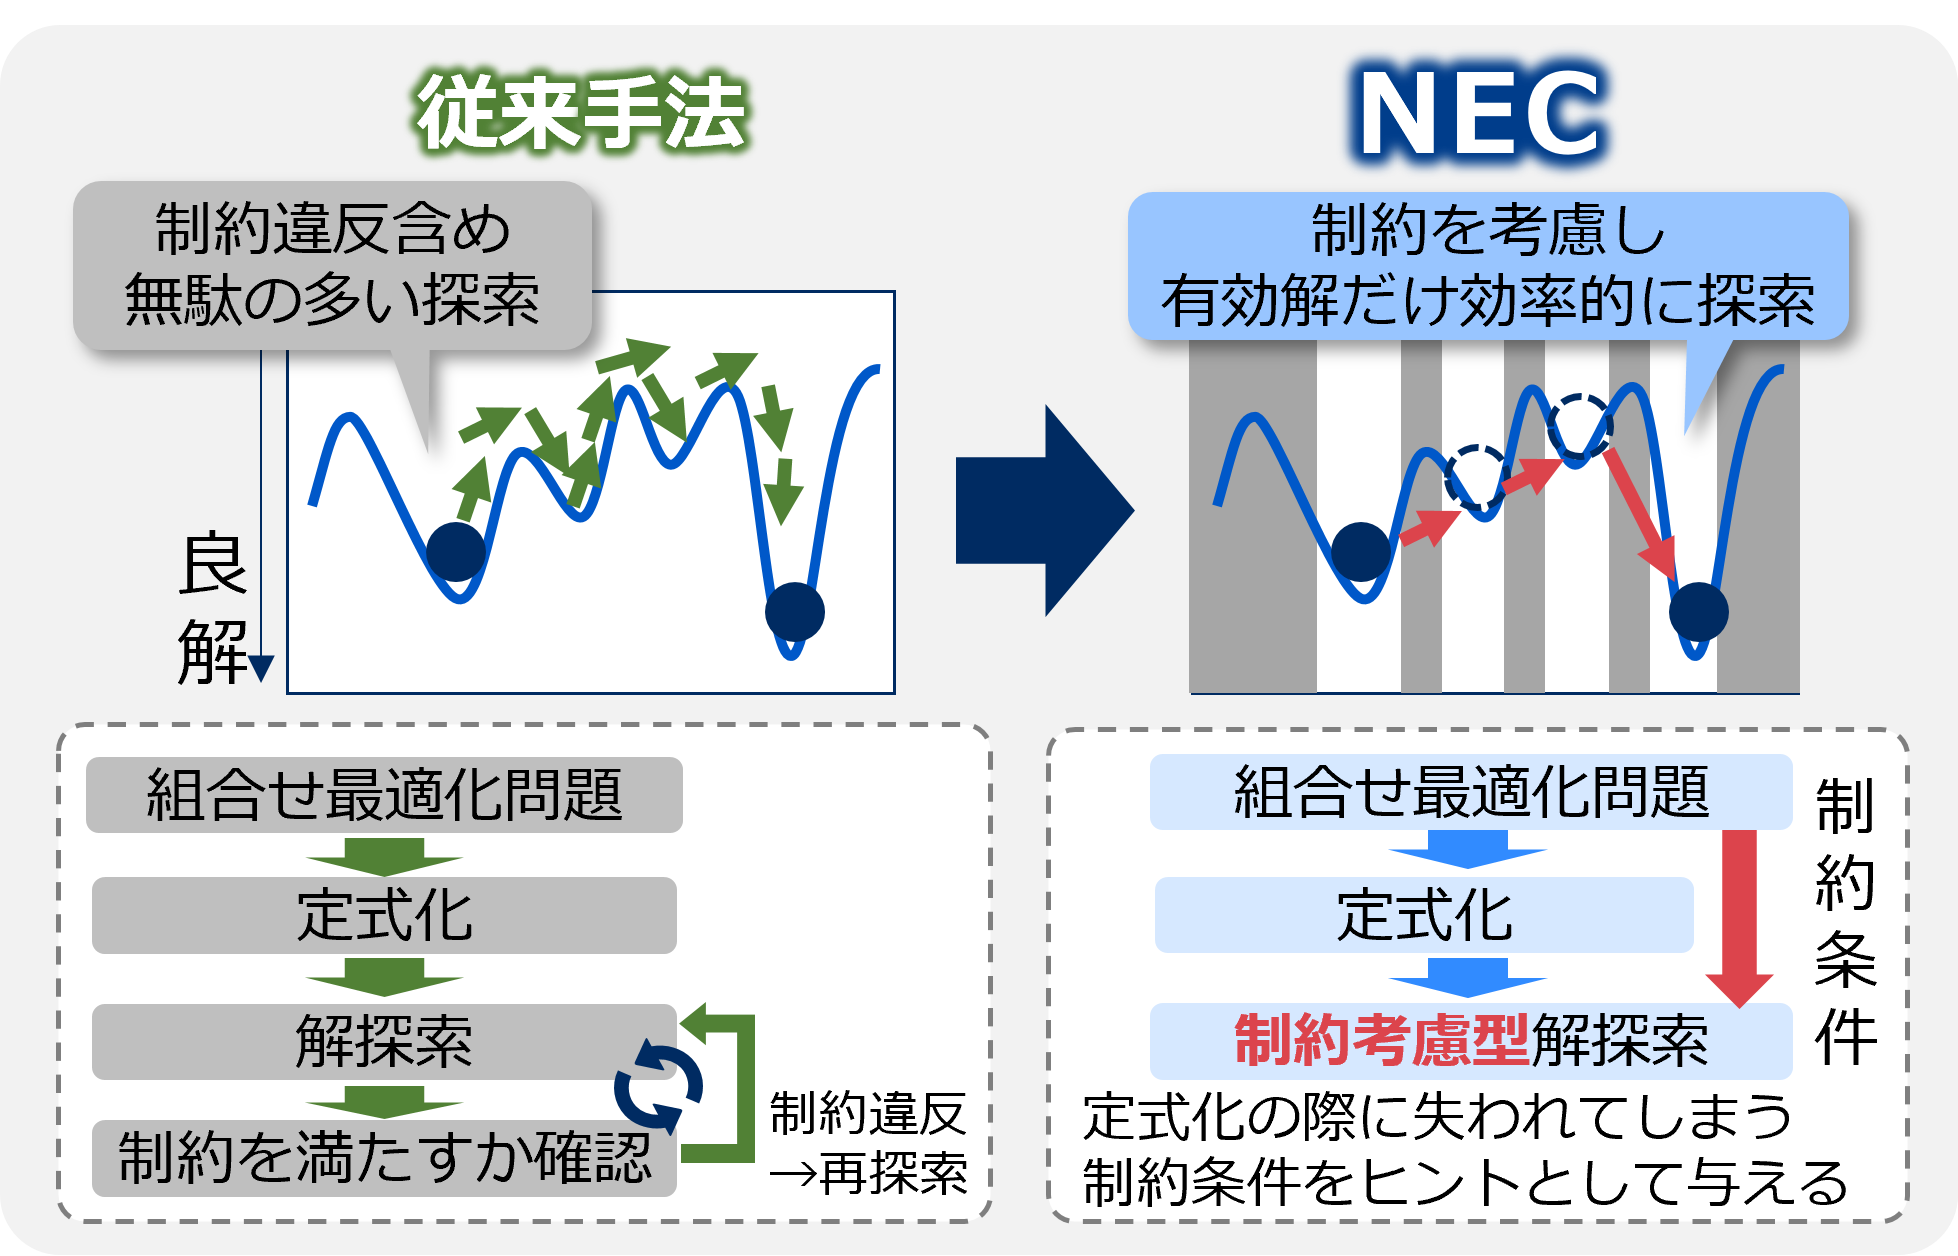
\includegraphics[bb=0 0 775 250, width=15cm]{NEC_VA_flip_option.png}
\caption{NEC VAによる制約を考慮した探索.}
\label{va_search}
\end{figure}

\begin{sourcecode}[h] % Figure環境と同様にhtbが使えます.pは使えません.
\caption{NEC VAのフリップオプションの使用例}\label{code:nec_va}
\begin{lstlisting}
# 制約条件の情報をリスト形式で定義
one_hot_list = [
    ['x[0][0]', 'x[0][1]', 'x[0][2]', 'x[0][3]'],
    ['x[1][0]', 'x[1][1]', 'x[1][2]', 'x[1][3]'],
    ['x[2][0]', 'x[2][1]', 'x[2][2]', 'x[2][3]'],
]

# モデル作成時に制約条件を入力
va_model = VectorAnnealing.model(qubo, offset, onehot=one_hot_list)
\end{lstlisting}
\vspace{5mm}
\end{sourcecode}

%4
\section{性能評価}

%4.1
\subsection{評価環境}
本評価では, 制約機能を有する擬似量子アニーリングマシンであるNEC VA, Fujitsu DA及び, 標準的な擬似量子アニーリングマシンとしてFixstars Amplify AEを評価用のソルバとして用いる. 各ソルバのスペックの一覧を表\ref{table_spec}に示す. Fujitsu DA及びFixstars Amplify AEは共にクラウド環境から利用可能であり, NEC VAはオンプレミス環境から利用可能である. このため, 評価ではFujitsu DA及びFixstars Amplify AEをクラウド環境からの実行とし, NEC VAはIntel Xeon Gold 6430が搭載されたオンプレミス環境からの実行とした. Fixstars Amplify AEは, API上では目的項と制約項を分離して入力できるものの, 制約項は内部で自動的にペナルティ関数へ変換されるのみであり, 制約を独立に処理する機構は実装されていない. 

ベンチマーク問題として, 制約を含まないMaxcut及び, 異なる制約を含む4つの最適化問題(QAP, TSP, QKP, MIS)を用いる. 制約機能を有するNEC VA, Fujitsu DAにおいては, 各制約に応じて適切な制約機能を指定する. 各問題において, 各ソルバで指定するパラメータ及び制約機能の一覧を表\ref{table_parameter}に示す. Fujitsu DAに特有の機能として, TSPやQAPで現れるツーウェイワンホット制約に特化したtwo\_way\_one\_hot\_groupsを指定できる. NEC VAにおいてフリップオプションを指定する場合, 実装方式の異なる二つの制約処理を選択することができる. speedモードでは, 外部入力された制約条件を探索時にヒント情報として活用し, 探索領域を制約を満たす解の近傍のみに絞って探索を行う. constraintモードでは, 外部入力された全ての制約条件を完全に満たす状態の中から解探索を行う. Fujitsu DAの制約機能及びNEC VAのconstraintモードを指定する場合, 制約項をQUBOに含める必要はない. Fixstars Amplify AE及びNEC VAのspeedモード実行では, 制約項の導入及び制約重みの設定が必要であり, 制約重みは各問題及び各ソルバに適した値を指定する必要がある. 各ソルバにおいて各問題で指定した制約重みの情報を表\ref{table_weight}に示す. 制約重みの決め方として, 実行した全ての試行で制約を満たす解が得られる重みのうち, 最小の値を選択した.

評価指標としてはTime to Solution (TTS)を使用し, 実行時間と解精度の観点から各制約の分類における制約機能の評価を行う. TTSはアニーリングの性能評価によく用いられる指標であり, 以下の式で表される.
\begin{equation}
{\rm{TTS}}(\tau, p_{R}) = \tau\frac{{\rm{ln}}(1-p_{R})}{{\rm{ln}}(1-p_{s}(\tau))} \label{tts_def}
\end{equation}
ここで, $\tau$は1回あたりの計算時間, $p_{R}$は$R$回の計算のうち1回でも指定精度の解を得る確率, $p_{s}(\tau)$は実際にその計算時間で指定精度の解を得た正答確率である. 評価では$p_{R}=0.99$, 即ちTTSを100回実行のうち少なくとも解を99回得るのに要する実行時間として定義する. また, TTSの基準とする解精度を各ベンチマーク問題に応じて指定する. ここで解精度は, 既知最適解における目的関数値からの誤差率を表す. 例えば解精度1\%とした場合, 最適解における目的関数値x1.01倍までの目的関数値が得られた場合を正答と見做す. 表\ref{table_target}に, 各ベンチマーク問題のインスタンス毎に指定した解精度を示す. 計算の実行回数として, NEC VAでは100, Fixstars Amplify AEでは10とし, Fujitsu DAでは, 目標のエネルギー値に到達した場合に自動的に計算を終了するtarget\_energyを指定して1回のみの実行とした. 

\newlength{\myheight}
\setlength{\myheight}{0.8cm}

\begin{table*}[htb]
\centering
  \caption{各疑似量子アニーリングマシンのスペック}
    \begin{tabular}{|c||c|c|c|c}
      \hline
      \parbox[c][\myheight][c]{0cm}{}
      & \parbox{10em}{Fixstars Amplify AE} & {NEC VA} & {Fujitsu DA}\\ \hline \hline
      求解方式 & Simulated Annealing & Simulated Annealing & MCMC Parallel Tempering\\ \hline
      提供形態 & クラウド & オンプレ & クラウド\\ \hline
      Hardware & Nvidia A100 & X86 CPU & GPU\\ \hline
      最大ビット/スピン数 & 262,144 & 10,0000+ & 10,0000+\\ \hline
      ビット階調 & 32bits/64bits & 64bits & 32bits/64bits\\ \hline
      制約処理技術 & - & 1hot & 2way-1hot\\ 
      {} & {} & 不等式制約 & 不等式制約\\ \hline
  \end{tabular}
\label{table_spec}
\end{table*}


\begin{table*}[htb]
\centering
  \caption{各疑似量子アニーリングマシンにおけるパラメータ設定}
    \begin{tabular}{|c||c|c|c|c|c|c|c|}
      \hline
      \parbox[c][\myheight][c]{0cm}{}
      & \parbox{10em}{Fixstars Amplify AE} & \multicolumn{4}{|c|}{NEC VA} & \multicolumn{2}{|c|}{Fujitsu DA}\\ \hline \hline
      & timeout[ミリ秒] & 始温度 & 終温度 & vector\_mode & 制約機能 & time\_limit\_sec[秒] & 制約機能\\ \hline 
      Maxcut & \multirow{2}{*}{$3000\sim900000$} & $5.0\sim10$ & $30\sim50$ & \multirow{2}{*}{speed} & - & $300\sim600$ & -\\
      \cline{1-1} \cline{3-3} \cline{4-4} \cline{6-6} \cline{7-7} \cline{8-8}
      TSP & & $10$ & $1000$ & & \multirow{2}{*}{onehot} & $5\sim1200$ & \multirow{2}{*}{two\_way\_one\_hot\_groups}\\
      \cline{1-1} \cline{2-2} \cline{3-3} \cline{4-4} \cline{5-5} \cline{7-7}
      QAP & \multirow{2}{*}{$5000\sim900000$} & 10 & 100 & \multirow{3}{*}{constraint} & & $60\sim300$ & \\
      \cline{1-1} \cline{3-3} \cline{4-4} \cline{6-6} \cline{7-7} \cline{8-8}
      QKP & & $0.1\sim5.0$ & $40\sim2000$ & & weighted\_sum & 5 & Inequalities\\
      \cline{1-1} \cline{2-2} \cline{3-3} \cline{4-4} \cline{6-6} \cline{7-7} \cline{8-8}
      MIS & 600000 & 10 & 100 & & andzero & 2 & PenaltyBinaryPolynomial\\ \hline
    \end{tabular}
\label{table_parameter}
\end{table*}

\begin{table}[tb]
\centering
  \caption{各ベンチマーク問題における制約重みの設定}
    \begin{tabular}{|c||c|c|c}
      \hline
      \parbox[c][\myheight][c]{0cm}{}
      & \parbox{10em}{Fixstars Amplify AE} & {NEC VA}\\ \hline \hline
      TSP & $0.1\alpha\sim0.5\alpha\,(\alpha={\rm Max}(d_{i,j}))$ & $0.04\alpha\sim0.05\alpha$\\ \hline
      QAP & $\beta\sim20\beta\,(\beta={\rm Max}(f_{i,j}d_{k,l}))$ & \multirow{3}{*}{-}\\
       \cline{1-1} \cline{2-2}
      QKP & \multirow{2}{*}{1.0} & \\
      \cline{1-1}
      MIS & & \\ \hline
  \end{tabular}
\label{table_weight}
\end{table}

\begin{table}[tb]
\centering
  \caption{各ベンチマーク問題におけるTTSの解精度}
    \begin{tabular}{|c||c|c|c|c|c|}
      \hline
      \multirow{2}{*}{Maxcut} & G11 & G32 & G65 & G72 & G81\\
      \cline{2-2} \cline{3-3} \cline{4-4} \cline{5-5} \cline{6-6}
                              & 最適解 & 0.5\% & \multicolumn{3}{|c|}{1\%}\\ \hline
      \multirow{2}{*}{TSP} & eil51 & kroA100 & ch150 & kroA200 & pr226\\
      \cline{2-2} \cline{3-3} \cline{4-4} \cline{5-5} \cline{6-6}
                              & 最適解 & 1\% & 5\% & 6\% & 20\%\\ \hline
      QAP                     & \multicolumn{5}{|c|}{全インスタンス1\%}\\ \hline
      QKP                     & \multicolumn{5}{|c|}{全インスタンス最適解}\\ \hline
      MIS                     & \multicolumn{5}{|c|}{全インスタンス最適解}\\ \hline
    \end{tabular}
\label{table_target}
\end{table}

%4.2
\subsection{結果・考察}

%4.2.1
\subsubsection{制約を含まないMaxcutによる評価}
% \textcolor{blue}{ベンチマークセットとして, Gset[YYY]のうち6つのインスタンス(G11, G32, G65, G72, G81)を用いた. 各インスタンス名の数値が大きくなるほど変数量が大きい.} TTS計算の基準とする解精度は, G11で0\%(最適解), G32で0.5\%, G65からG81では1\%とした. \textcolor{blue}{ソルバ毎の設定として, NEC VAではコア数を40, 始温度を5-10, 終温度を30-50, num\_sweepsを2000-8000, speedモードによる実行とし, 富士通DAではtime\_limit\_secを300-600, target\_energyを問題毎に設定した解精度のエネルギー, Fixstars Amplify AEではtimeoutを3000-900000(msec)とした.}

図\ref{Maxcut_TTS}に, MaxcutによるTTSの評価結果を示す. ベンチマークセットとして, Gset\cite{gset}のうち5つのインスタンスを用いた. 各インスタンス名の数値が大きいほど変数量が大きい. 図\ref{Maxcut_TTS}より, 全インスタンスにおいてNEC VA, Fixstars Amplify AE, Fujitsu DAの順にTTSが小さい. 図\ref{Maxcut_Time_Cost}には, 最大規模であるG81で測定した実行時間と解精度の関係を示す. Fixstars Amplify AE及びFujitsu DAでは実行時間の上限を指定するtimeout及びtime\_limit\_secを指定し, NEC VAではアニーリングの試行回数に相当するnum\_sweepsを調整することにより, 異なる4パターンの実行時間で得られた最終的な解の目的関数値を示している. 目的関数値は, 各データセットの既知最適解によって正規化されており, 値が1に近付くほど最適解に近いことを表す. 図\ref{Maxcut_Time_Cost}より, NEC VAが4.7[sec]以降の実行時間では最も精度が高く, 測定した最長の実行時間である105[sec]では0.3\%精度の解まで到達している. 

Maxcutでは, NEC VA及びFujitsu DAによる制約機能は使用されておらず, 上記の性能差は主に各ソルバのプラットフォームであるHWの性能差やアニーリングアルゴリズムの実装の違いに起因するものと考えられる.

\begin{figure}[hb]
\centering
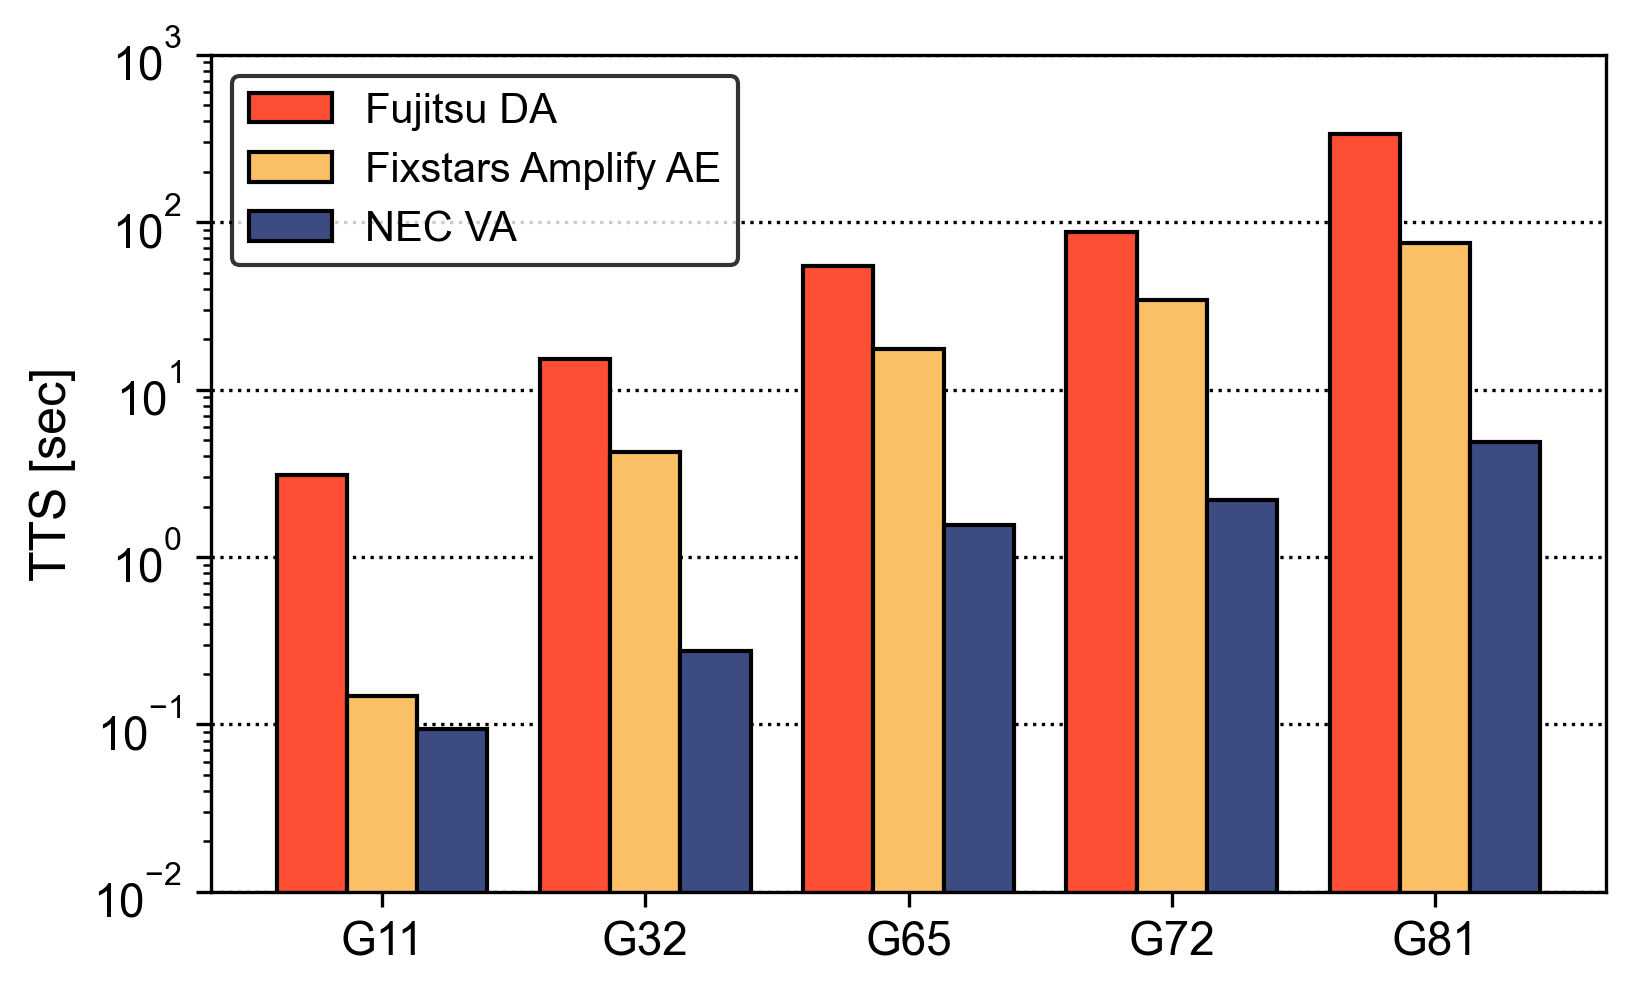
\includegraphics[bb=0 0 700 250, width=15cm]{TTS_Maxcut.png}
\caption{MaxcutにおけるTTSの比較.}
\label{Maxcut_TTS}
\end{figure}

\begin{figure}[hb]
\centering
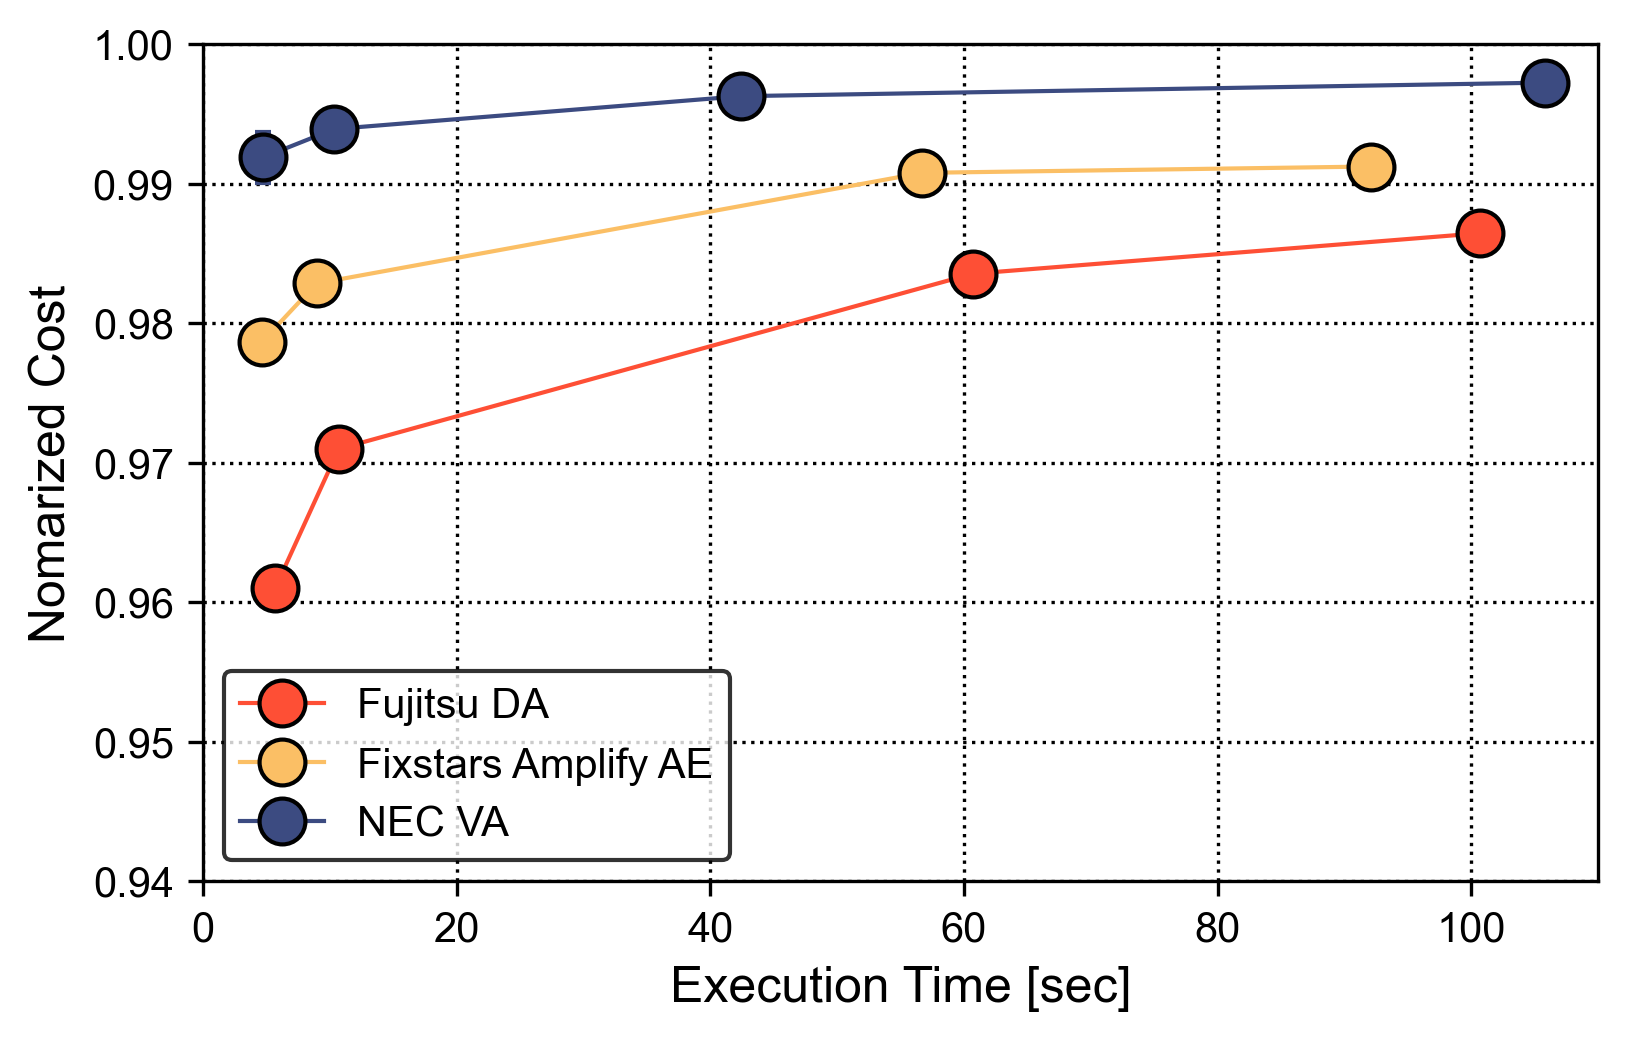
\includegraphics[bb=0 0 700 250, width=15cm]{Energy_Maxcut.png}
\caption{Maxcutにおける実行時間と解精度の関係.}
\label{Maxcut_Time_Cost}
\end{figure}

%4.2.2
\subsubsection{ワンホット制約を持つTSP, QAPによる評価}
% \textcolor{blue}{TSPのベンチマークセットとして, TSPLIB[YYY]のうち5つのインスタンス(eil51, kroA100, ch150, kroA200, pr226)を用いた. 各インスタンス名の数値はTSPの都市数を表し, 数値が大きいほど変数量が大きい. TTS計算の基準とする解精度(最適解からの誤差)はeil51で0\%(最適解), kroA100で1\%, ch150で5\%, kroA200で6\%, pr226で20\%とした. ソルバ毎の設定として, NEC VAではコア数を40, 始温度を5-10, 終温度を30-50, num\_sweepsを2000-8000, speedモードによる実行とし, 富士通DAではtime\_limit\_secを300-600, target\_energyを問題毎に設定した解精度のエネルギー, Fixstars Amplify AEではtimeoutを3000-900000(msec)とした. QAPのベンチマークセットとして, QAPLIB[ZZZ]のうち6つのインスタンス(tai12b, tai20b, tai50b, tai80b, tai100b, tai150b)を用いた. 各インスタンス名の数値が大きくなるほど変数量が大きい. TTS計算の基準とする解精度は全てのインスタンスに対して1\%とした. ソルバ毎の設定として, NEC VAではコア数を40, 始温度を10, 終温度を100, num\_sweepsを10-800, onehotフリップオプションを有効化, constraintモードによる実行とし, 富士通DAではtime\_limit\_secを60-300, target\_energyを最適解のエネルギー*1.01, 制約項をtwo\_way\_one\_hot\_groupsにより指定し, Fixstars Amplify AEではtimeoutを5000-900000(msec), 制約項の重みを距離行列と輸送量行列の積の最大値の1.0-20倍とした.}

図\ref{TSP_TTS},\ref{QAP_TTS}に, TSP, QAPによるTTSの評価結果を示す. TSPのベンチマークセットとして, TSPLIB\cite{tsplib}のうち5つのインスタンスを使用し, QAPのベンチマークセットとして, QAPLIB\cite{qaplib}のうち6つのインスタンスを使用した. 各インスタンス名の数値は地点数を表し, 数値が大きいほど変数量が大きい. 図\ref{TSP_TTS}より, TSP100地点までの小中規模ではFixstars Amplify AE, Fujitsu DA, NEC VAの順に小さいTTSとなるが, 150地点を超える大規模ではFixstars Amplify AE, Fujitsu DAにおける実行時間が増大し, NEC VAが最小のTTSとなる. 一方, 図\ref{QAP_TTS}より, QAPではtai12bを除く全てのインスタンスでFujitsu DAが最小のTTSを達成している. Fixstars Amplify AEでは大規模において実行時間が増大し, グラフが表示されていない最大のtai150bでは指定精度の解が得られていない. 大規模でFixstars Amplify AEの性能が低下している要因として, 内部で自動的に導入されたペナルティ関数によりQUBO全体のエネルギー地形が複雑化したことに加えて, 大規模では制約を満たすために大きな制約重みを指定したことが探索精度に影響を与えたと考えられる. 

図\ref{TSP_Time_Cost},\ref{QAP_Time_Cost}には, TSP, QAPそれぞれの最大のインスタンスであるpr226, tai150bで測定した実行時間と解精度の関係を示す. 図\ref{TSP_Time_Cost}より, TSP pr226において実行時間600[sec]以内ではNEC VAが最も精度が高く, 測定した最長の597[sec]では8.6\%精度まで到達している. 一方, 図\ref{QAP_Time_Cost}より, QAP tai150bではFujitsu DAが実行時間43[sec]を超えた時点で解精度が大きく向上し, 最長の132[sec]では0.3\%精度まで到達している. NEC VAは最短の14[sec]時点で2\%精度まで到達するものの, その後は精度の向上が頭打ちとなる傾向が見られ, 最長の98[sec]では0.8\%精度への到達に留まっている.

上記の結果より, ツーウェイワンホット制約を含むTSP, QAPにおいては, NEC VA, Fujitsu DAがFixstars Amplify AEに対して高い性能を示していることが分かる. これは, 前節のMaxcutの結果と比較して異なる性能傾向を示すものであり, 制約機能が求解性能に大きく寄与していることを示唆している. また, NEC VA, Fujitsu DAの結果に着目すると, 同一の制約を含むTSP, QAPにおいて, これら二つのソルバの性能差が逆転していることが分かる. この要因として, 各問題の特性や各ソルバの制約処理の実装の違いが影響していると考えられる. 図\ref{TSP_energy_landscape}, \ref{QAP_energy_landscape}に, TSP, QAPの3地点のデータにおける, 解候補となる全スピン状態に対して目的関数のエネルギー値をプロットした分布を示す. 各エネルギー分布を比較すると, TSPではエネルギー値が近いスピン状態が広範囲に点在している傾向が見られる一方, QAPではエネルギー値が近いスピン状態が局所的に分布している領域が存在していることが分かる. 図\ref{TSP_speed_vs_const}, \ref{QAP_speed_vs_const}には, TSP, QAPにおける, NEC VAの異なる制約処理機能であるspeedモード, constraintモードで実行した場合の同一実行時間での正規化された解精度分布を示す. 図\ref{TSP_speed_vs_const}, \ref{QAP_speed_vs_const}より, TSPにおいてはspeedモードによる実行, QAPにおいてはconstraintモードによる実行がそれぞれ同一実行時間では高精度な解に到達していることが分かる. speedモード及びconstraintモードの実装上の違いとして, speedモードでは外部入力された制約条件を考慮しつつ比較的広範囲である解空間の中から解探索を行う一方, constraintモードでは外部入力された全ての制約条件を完全に満たす局所的な解空間の中から解探索を行う. このため, 最適解に近いエネルギー値が広範囲に分布するTSPではspeedモードによる実行で高精度の解が得られ, 最適解に近いエネルギー値が局所的に分布するQAPではconstraintモードによる実行で高精度の解が得られたと考えられる. Fujitsu DAの制約機能であるtwo\_way\_one\_hot\_groupsを指定した場合, 解の探索過程においてツーウェイワンホット制約を満たすよう, 一つの変数を反転すると同時に他の三つの変数が自動的に更新される. これはNEC VAにおける一次元のonehotフリップオプションを指定する場合と比較して, より局所的な解空間の中での解探索となることから, TSP, QAPの評価結果においてNEC VAとFujitsu DAが上記と同様の性能傾向を示したものと考えられる.

\begin{figure}[hb]
\centering
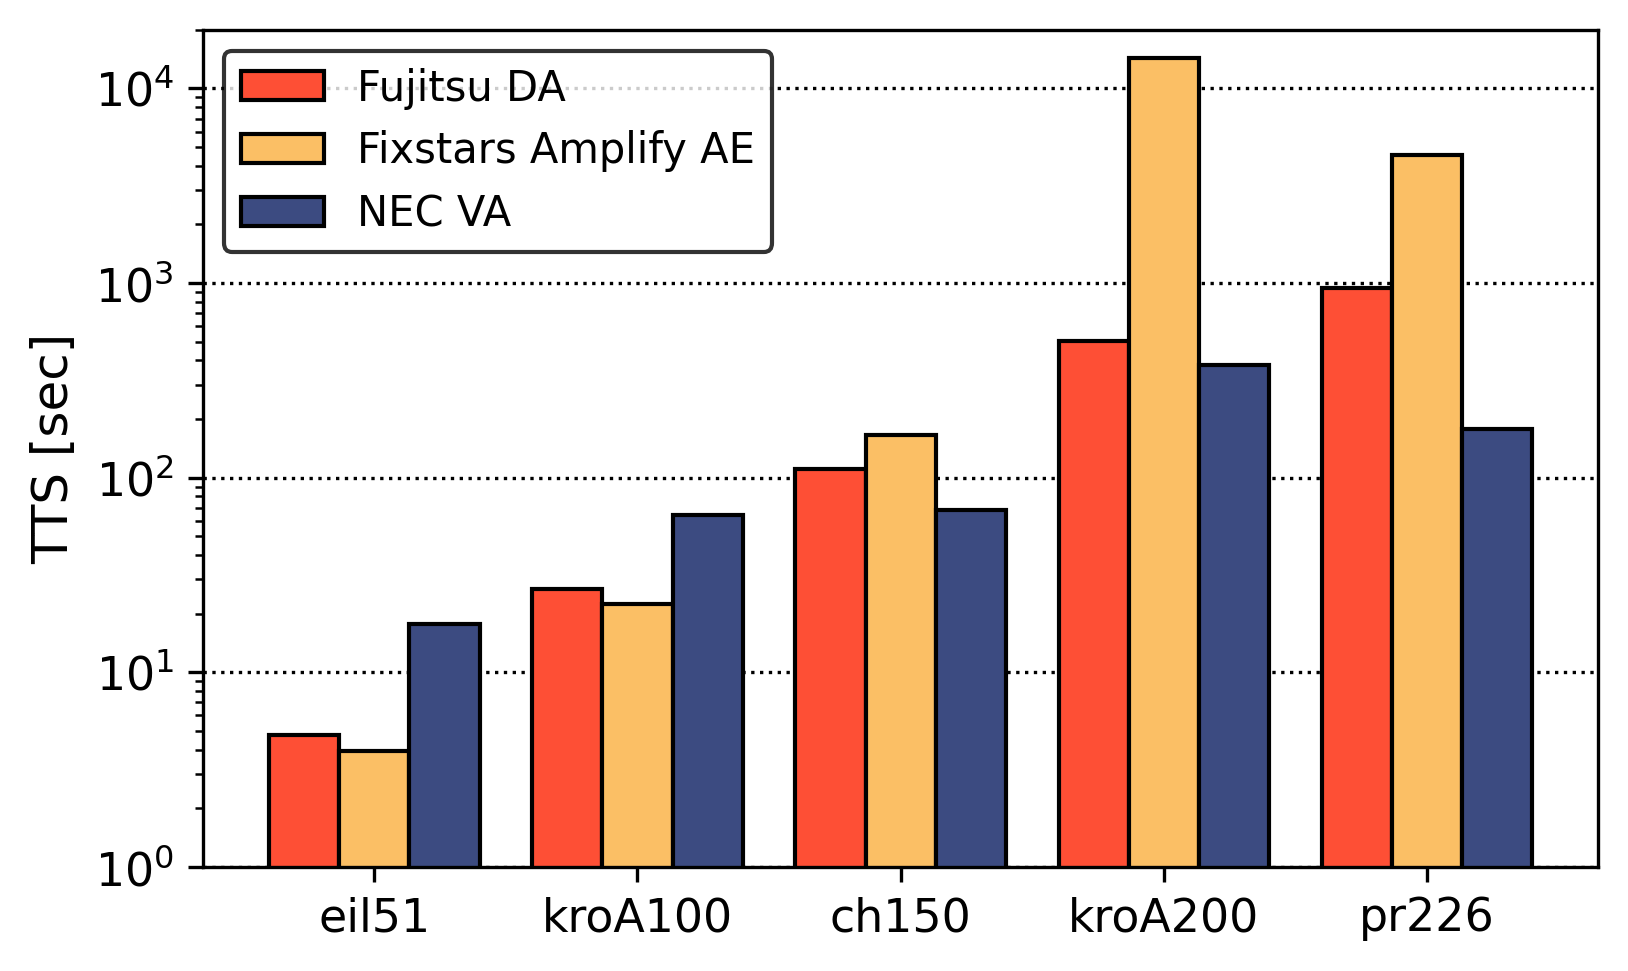
\includegraphics[bb=0 0 700 250, width=15cm]{TTS_TSP.png}
\caption{TSPにおけるTTSの比較.}
\label{TSP_TTS}
\end{figure}

\begin{figure}[hb]
\centering
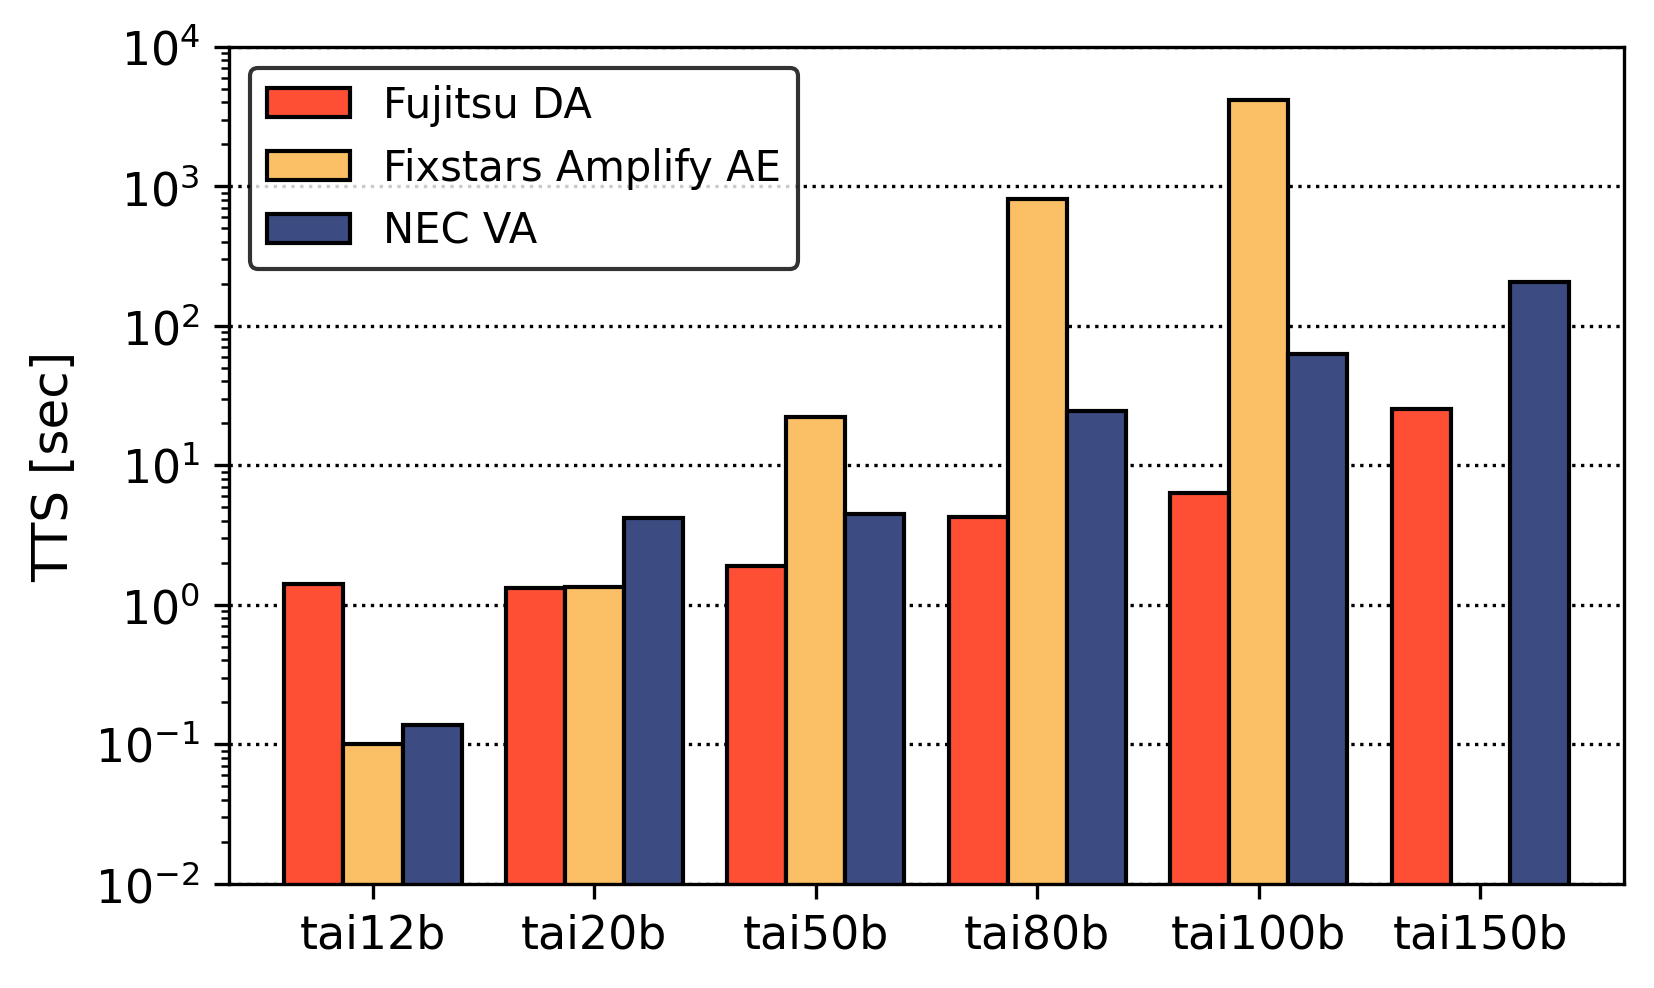
\includegraphics[bb=0 0 700 250, width=15cm]{TTS_QAP.png}
\caption{QAPにおけるTTSの比較.}
\label{QAP_TTS}
\end{figure}

\begin{figure}[hb]
\centering
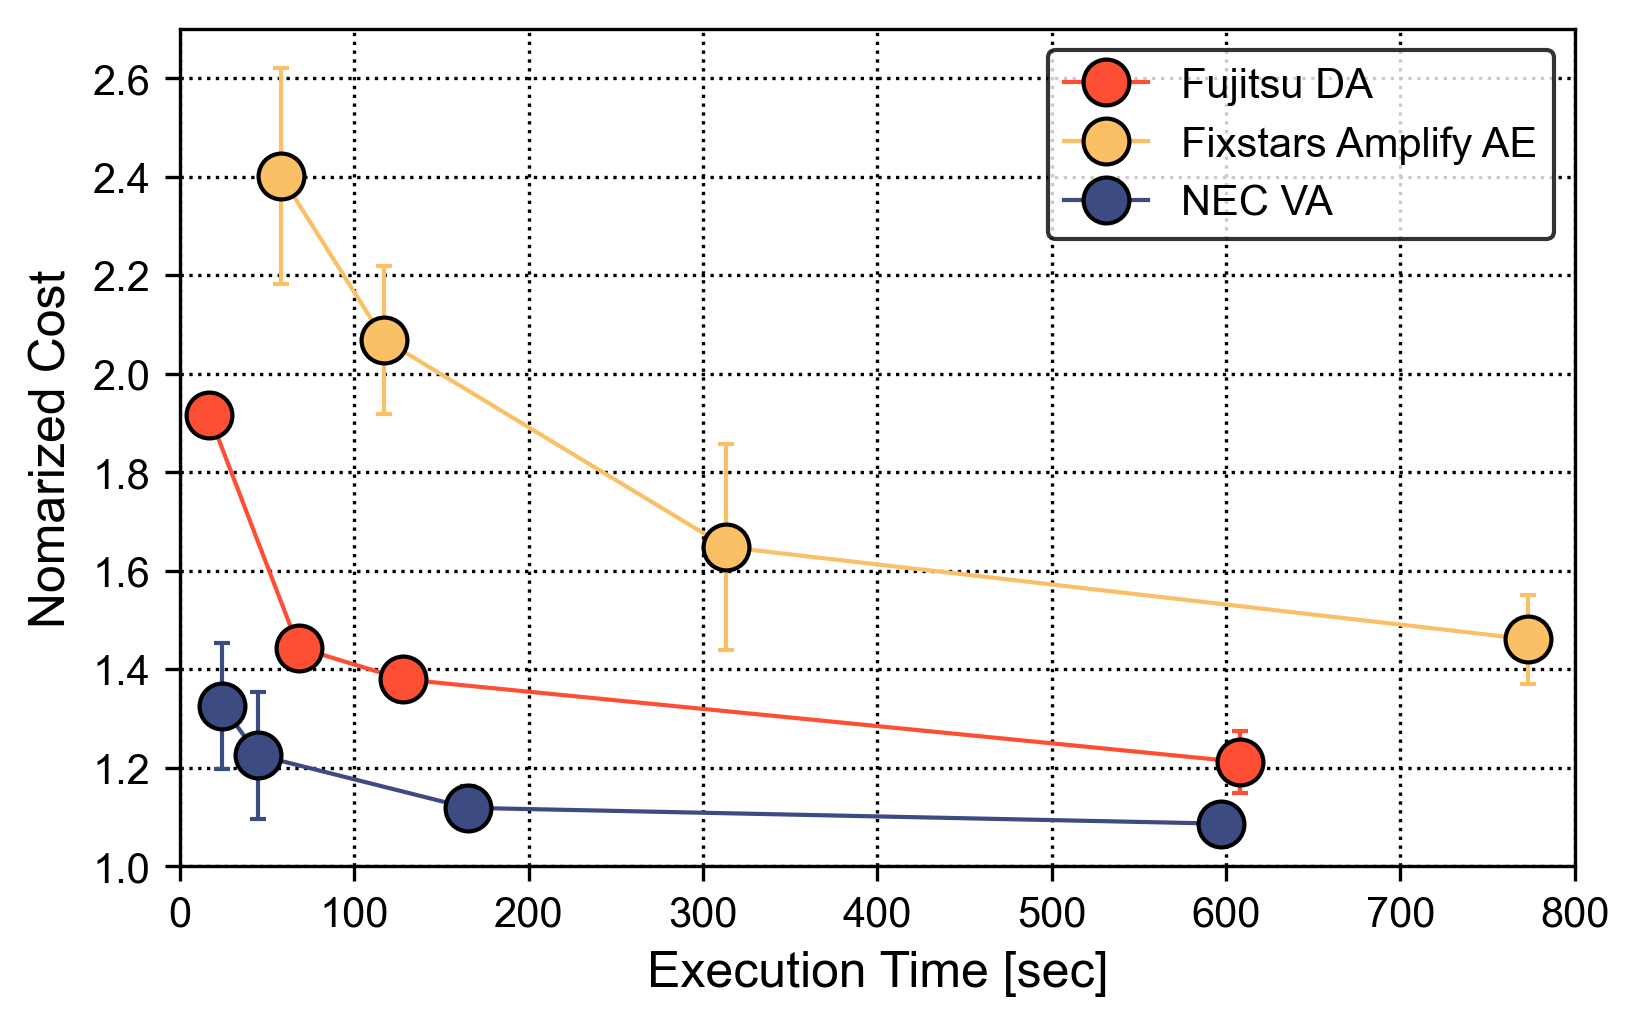
\includegraphics[bb=0 0 700 250, width=15cm]{Energy_TSP.png}
\caption{TSPにおける実行時間と解精度の関係.}
\label{TSP_Time_Cost}
\end{figure}

\begin{figure}[hb]
\centering
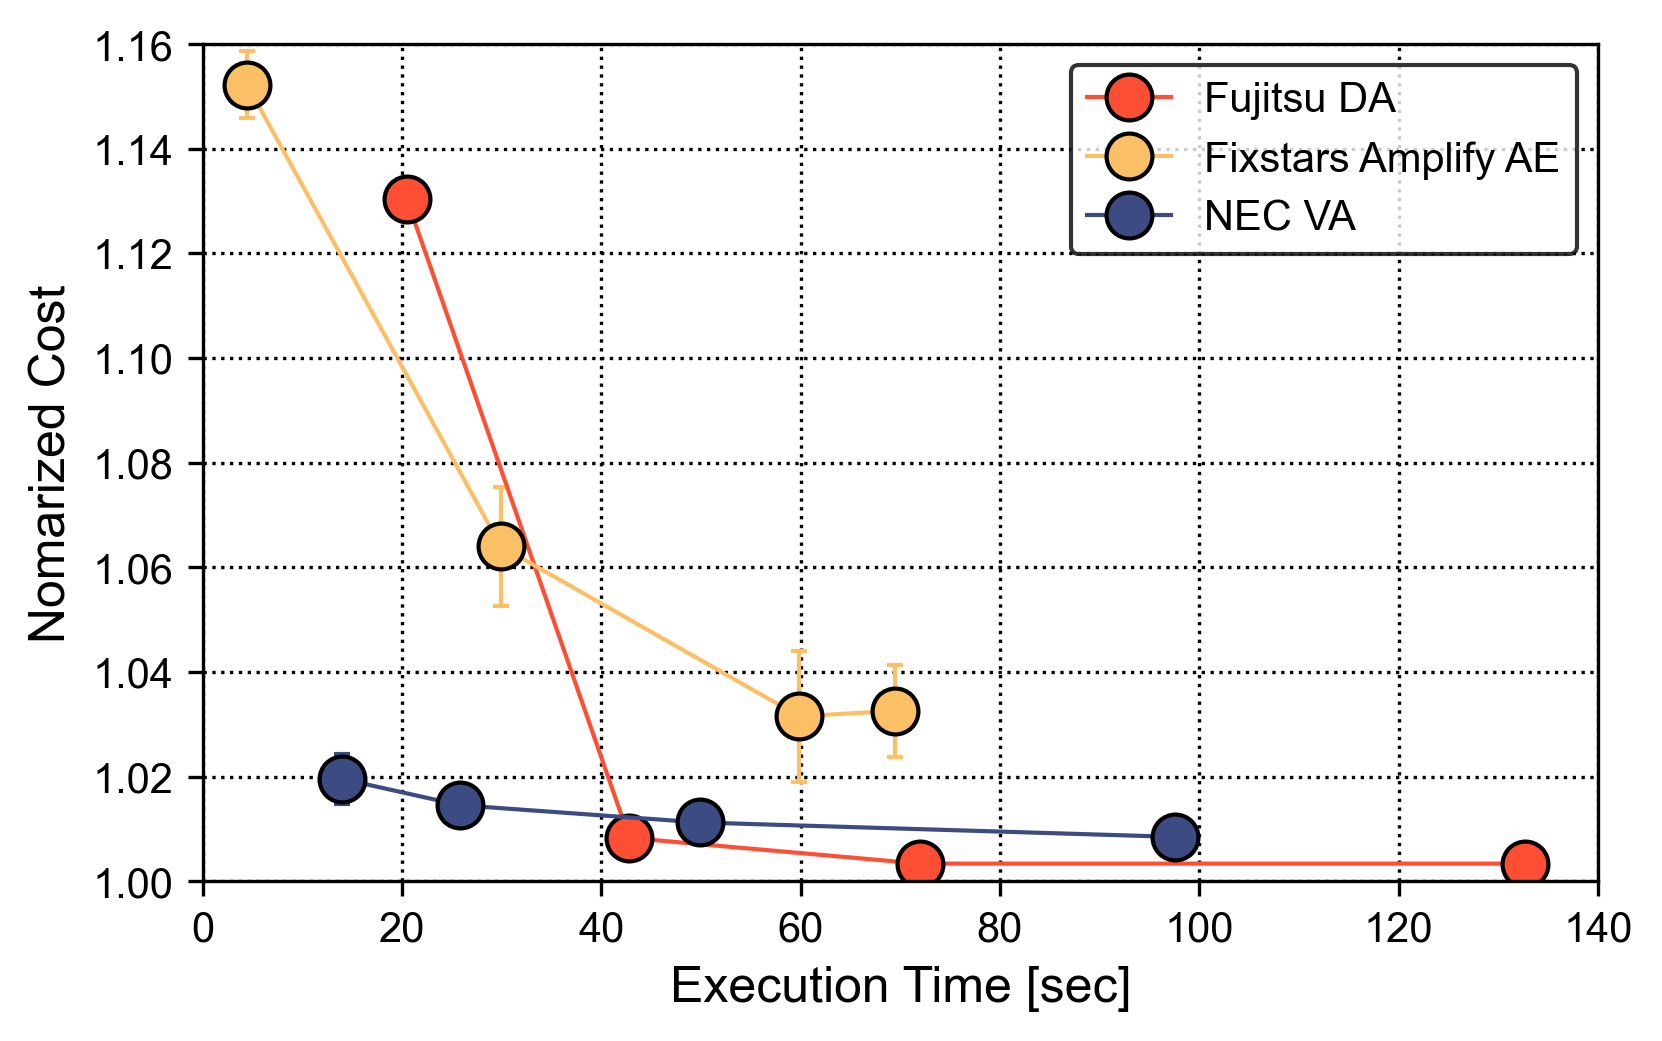
\includegraphics[bb=0 0 700 250, width=15cm]{Energy_QAP.png}
\caption{QAPにおける実行時間と解精度の関係.}
\label{QAP_Time_Cost}
\end{figure}

\begin{figure}[hb]
\centering
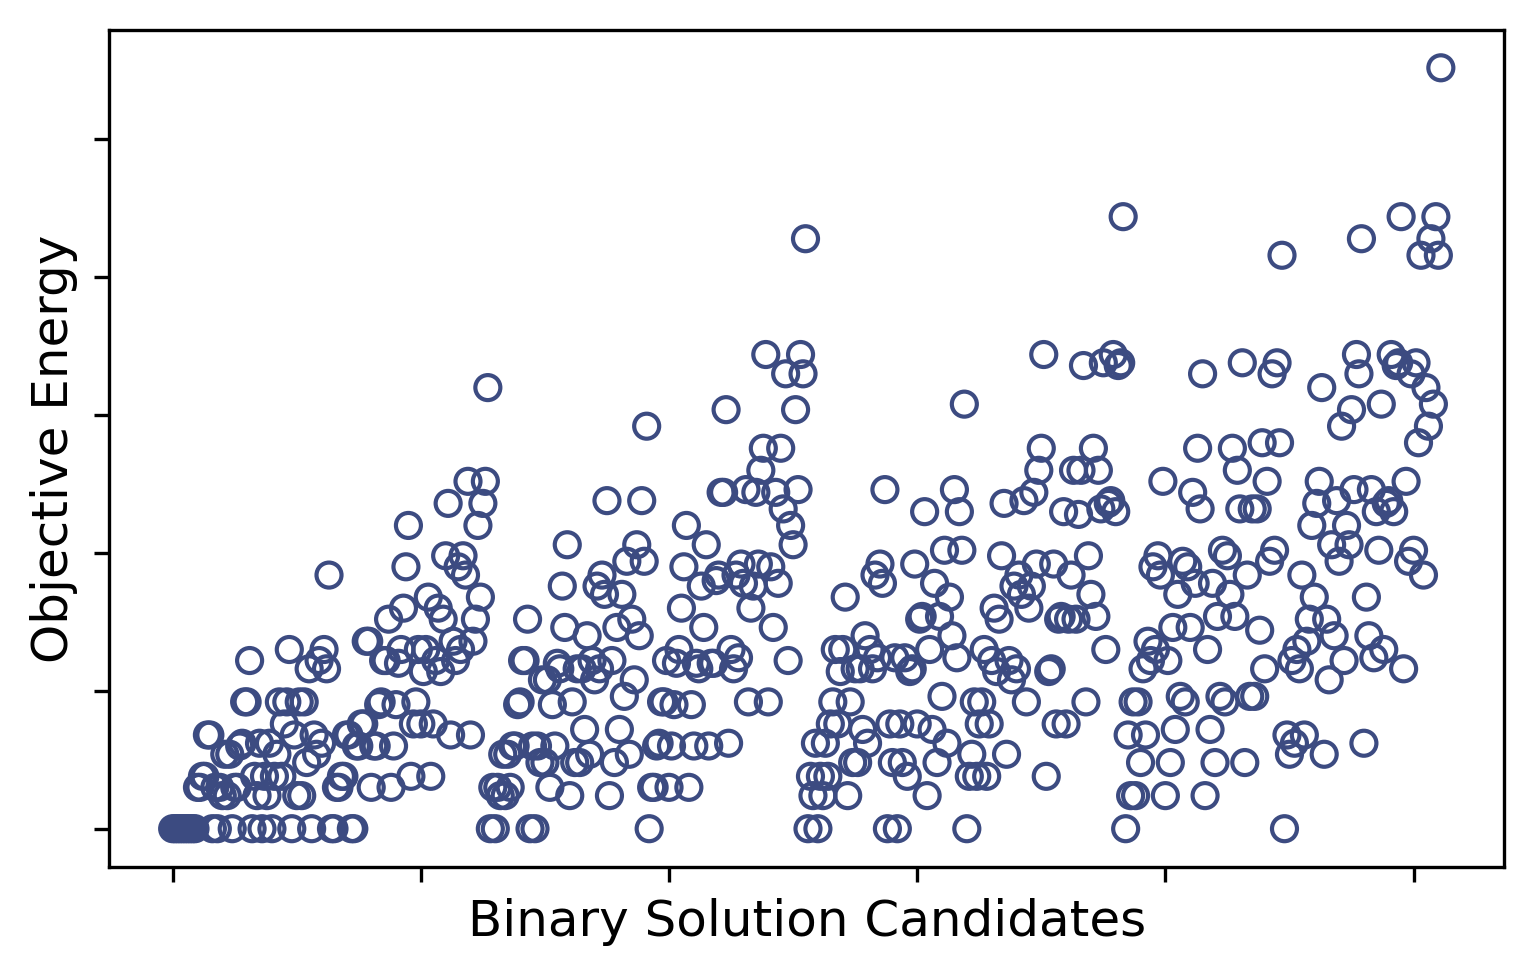
\includegraphics[bb=0 0 700 250, width=15cm]{Energy_Landscape_TSP.png}
\caption{3地点TSPにおける全スピン状態のエネルギー分布.}
\label{TSP_energy_landscape}
\end{figure}

\begin{figure}[hb]
\centering
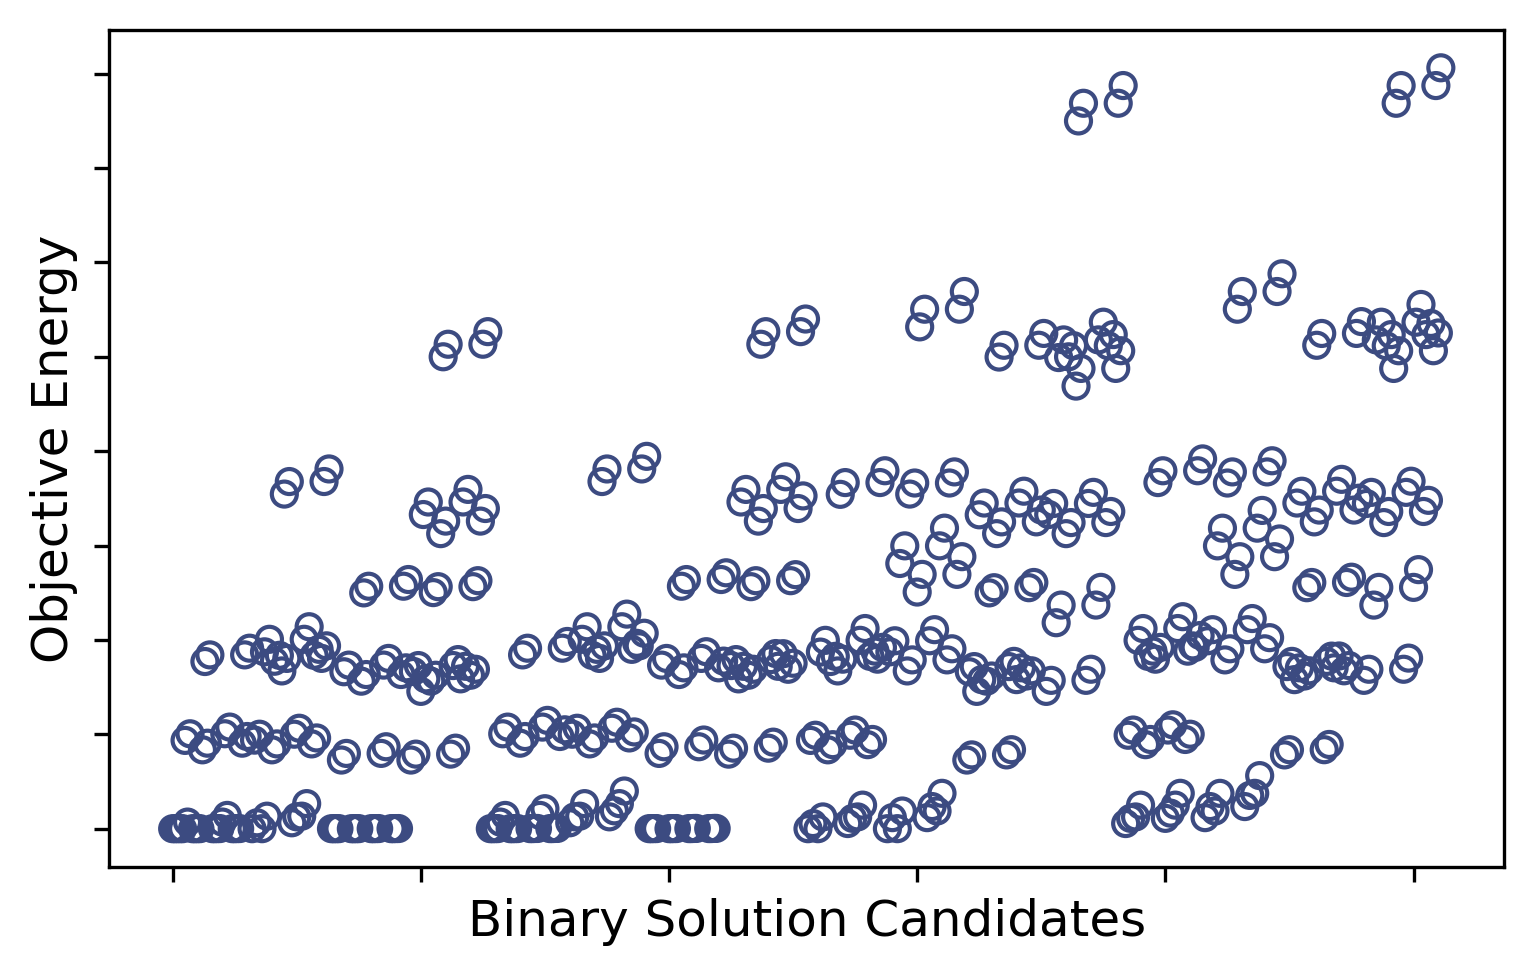
\includegraphics[bb=0 0 700 250, width=15cm]{Energy_Landscape_QAP.png}
\caption{3地点QAPにおける全スピン状態のエネルギー分布.}
\label{QAP_energy_landscape}
\end{figure}

\begin{figure}[hb]
\centering
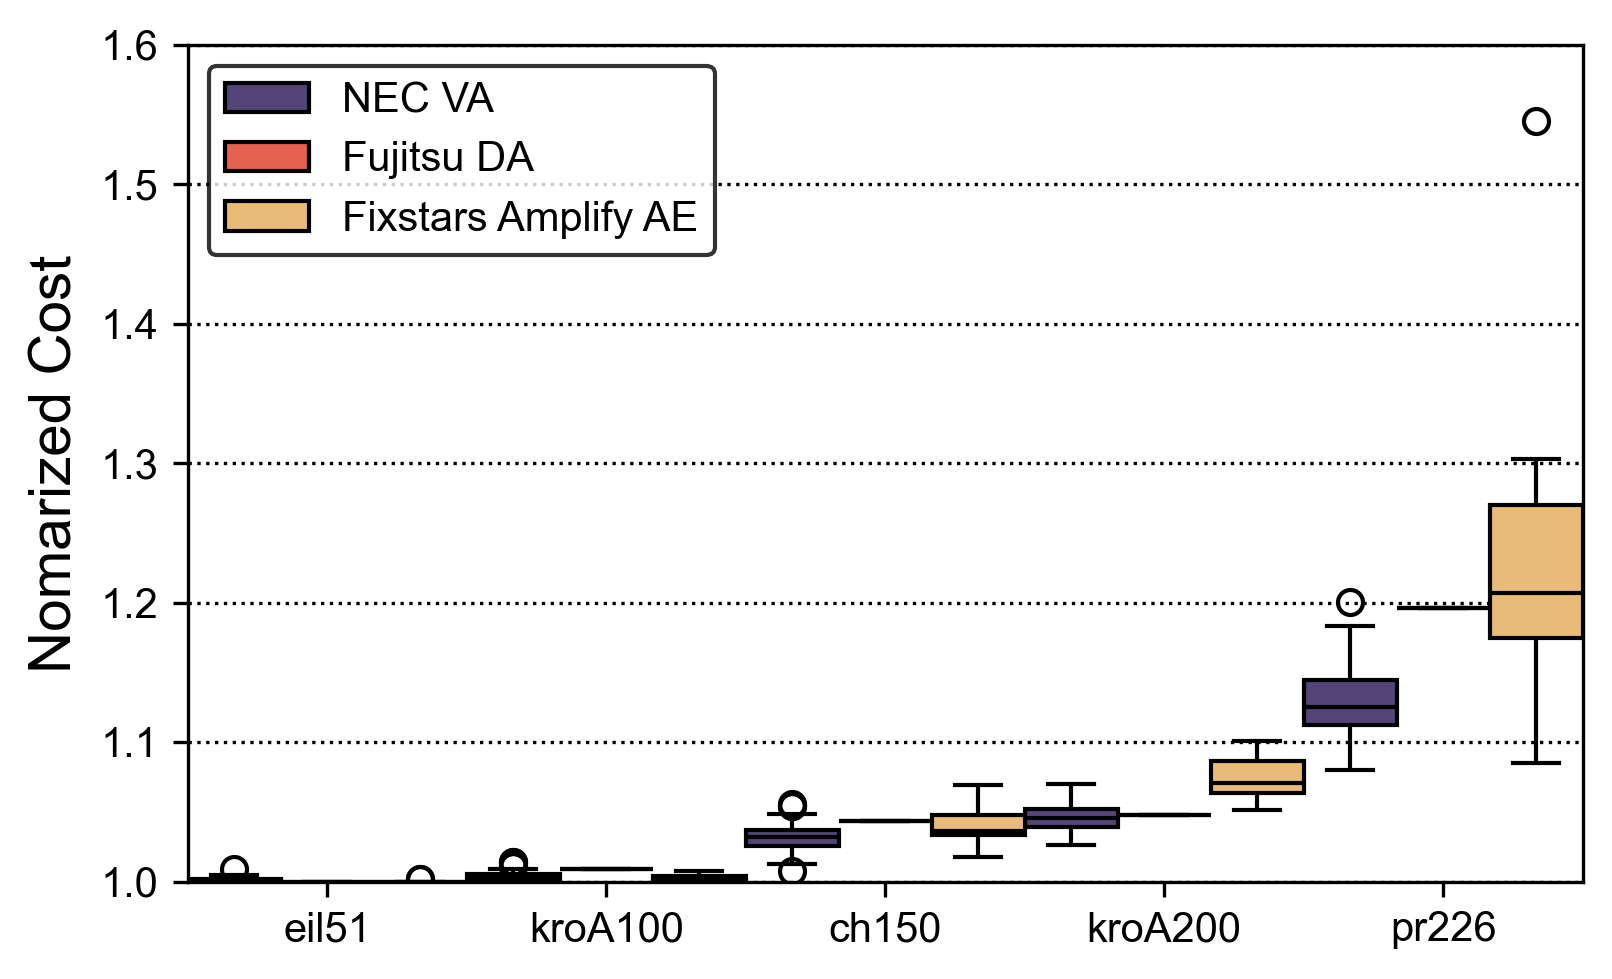
\includegraphics[bb=0 0 700 250, width=15cm]{speed_vs_constraint_TSP.png}
\caption{TSPにおけるNEC VAの2種類の制約機能の性能比較.}
\label{TSP_speed_vs_const}
\end{figure}

\begin{figure}[hb]
\centering
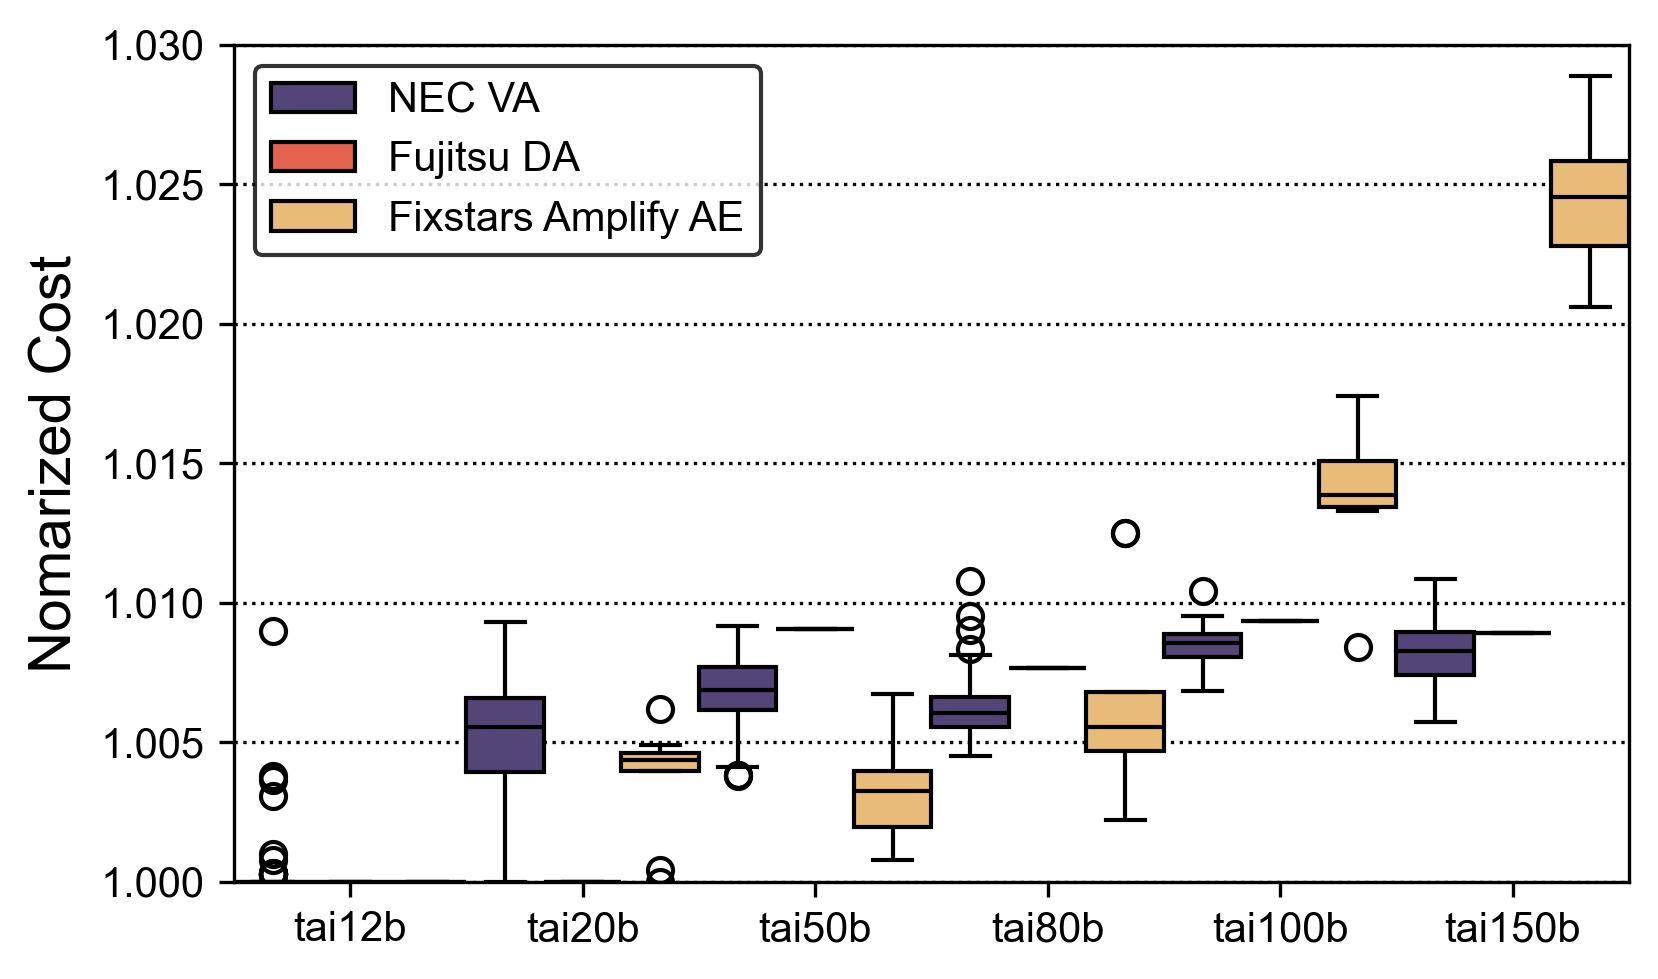
\includegraphics[bb=0 0 700 250, width=15cm]{speed_vs_constraint_QAP.png}
\caption{QAPにおけるNEC VAの2種類の制約機能の性能比較.}
\label{QAP_speed_vs_const}
\end{figure}

%4.2.3
\subsubsection{不等式制約を持つQKPによる評価}
% \textcolor{blue}{ベンチマークセットとして, 先行研究[YYY]で作成されたQKPインスタンスのうち10のインスタンスを用いた. 各インスタンス名の\_に続く最初の数値は変数量, その次の数値は密度を表す. 例えば, jeu\_100\_25\_1は100変数, 結合密度25%のインスタンスである. TTS計算の基準とする解精度は, 全てのインスタンスで最適解とした. ソルバ毎の設定として, NEC VAではコア数を40, 始温度を0.1-5.0, 終温度を40-2000, num\_sweepsを5-60000, weighted\_sumフリップオプションを有効化, constraintモードによる実行とし, 富士通DAではtime\_limit\_secを5, target\_energyを最適解のエネルギー, 制約項をInqualitiesにより指定し, Fixstars Amplify AEではtimeoutを5000-900000(msec), 制約項の重みを1.0とした.}

図\ref{QKP_TTS}に, QKPによるTTSの評価結果を示す. ベンチマークセットとして, 先行研究\cite{qkplib}で作成されたQKPインスタンスのうち10のインスタンスを用いた. 各インスタンス名の\_に続く最初の数値は変数量, その次の数値はQUBOの結合密度を表す. 例えば, jeu\_100\_25\_1は100変数, 結合密度25%のインスタンスである. 図\ref{QKP_TTS}において, TTSの結果が表示されていないインスタンスでは最適解が得られていない. 図\ref{QKP_TTS}より, Fixstars Amplify AEでは10問中6問で最適解が得られておらず, NEC VAでは10問中2問では最適解が得られていない. また, Fixstars Amplify AE, NEC VAでは各インスタンスの変数量やQUBOの結合密度とは独立にTTSがばらつく傾向が見られる. TTSにばらつきが生じる要因として, 各インスタンスのQUBO固有のエネルギー地形の複雑さが探索精度に影響を与えたと考えられる. 一方, Fujitsu DAでは全インスタンスで3秒以内のTTSで最適解に到達している. \textcolor{blue}{Fujitsu DAの性能の考察が必要.}
制約機能を持たないFixstars Amplify AEでは, 内部で不等式制約からペナルティ関数が生成される過程で補助変数が自動的に追加されるため, QUBOに目的関数のみを含むNEC VA, Fujitsu DAと比較して解空間が複雑化し, 探索精度に影響を与えることが予想される. 実際に図\ref{QKP_TTS}より, Fixstars Amplify AEでは, 過半数のインスタンスで最適解が得られておらず, NEC VA, Fujitsu DAと比較して求解精度が低下していることが分かる. 

不等式制約をペナルティ関数として導入する場合の性能への影響の評価として, NEC VAを用いて, フリップオプションを使用せず, 不等式制約をペナルティ関数として導入した場合の性能を確認する. 図\ref{QKP_speed_vs_const}には, QKPの各インスタンスにおいて, NEC VAによるconstraintモードを指定した場合の実行, 及びペナルティ関数を導入して実行した場合の同一実行時間における正規化された解精度分布を示す. 図\ref{QKP_speed_vs_const}より, ペナルティ関数が含まれないconstraintモードによる実行では, 全インスタンスで最適解もしくは最適解近傍に分布しているのに対して, ペナルティ関数を導入した場合の実行では, 最適解の0.1倍から0.9倍の精度に分布している. このことから, 不等式制約をペナルティ関数として含めることで性能に大きな影響を与える一方で, 制約機能を使用することでペナルティ関数の導入を回避し, 高い求解性能を実現できることが分かる.

\begin{figure}[hb]
\centering
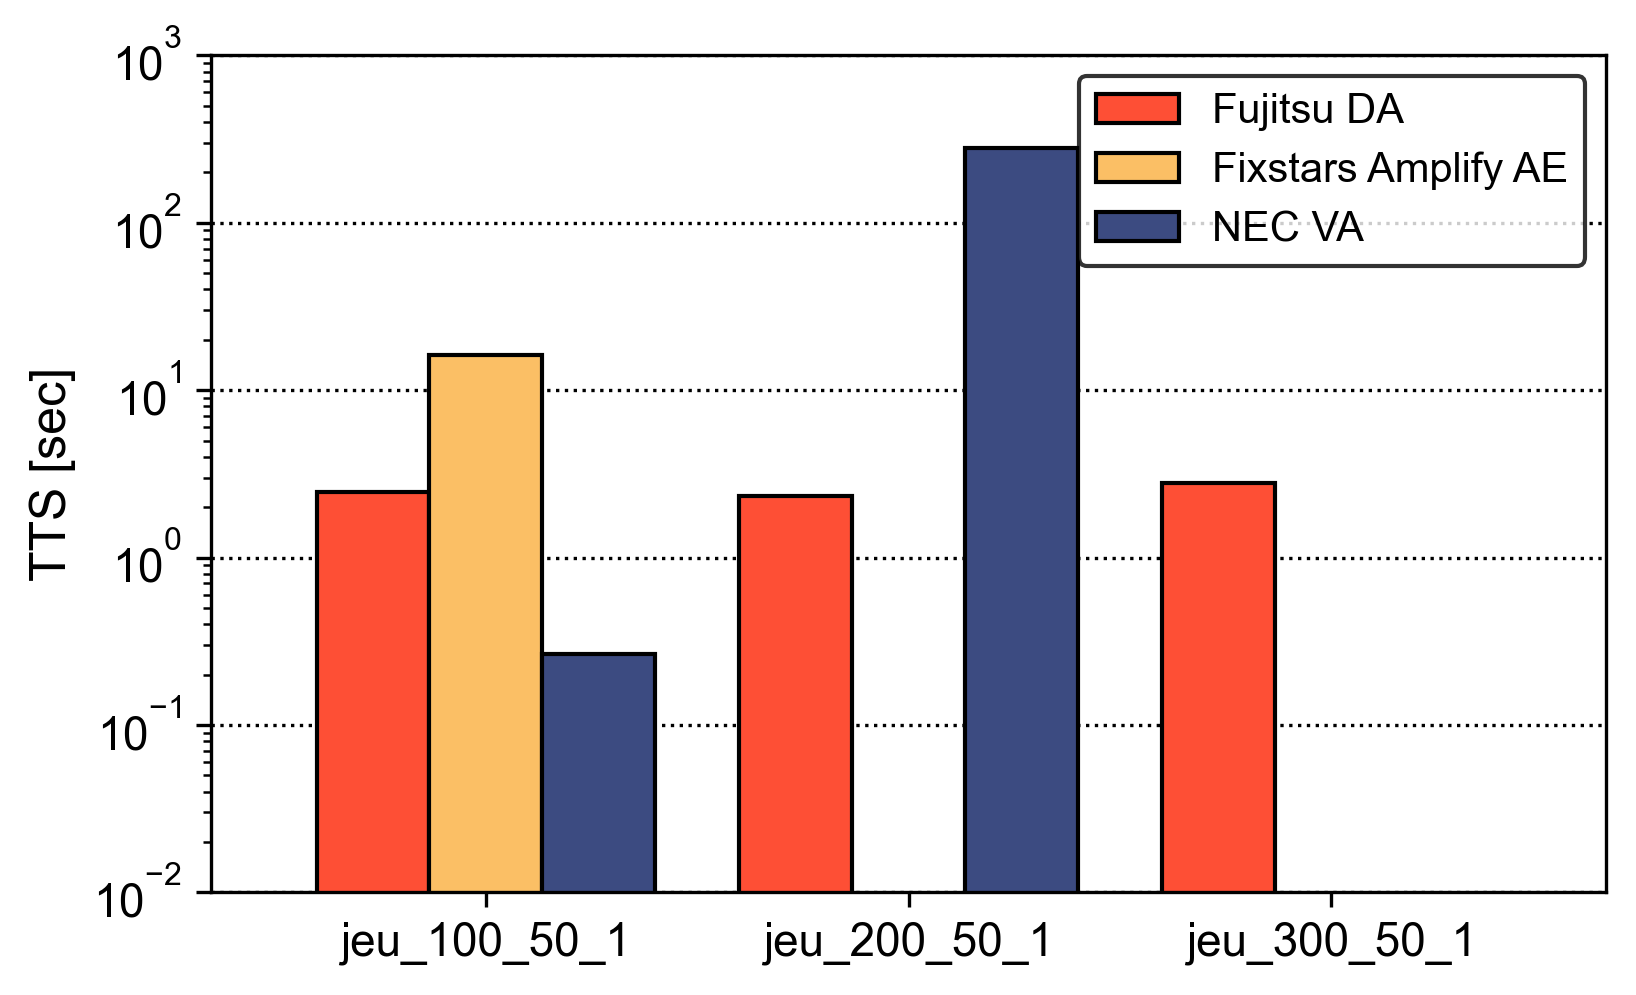
\includegraphics[bb=0 0 700 280, width=15cm]{TTS_QKP.png}
\caption{QKPにおけるTTSの比較.}
\label{QKP_TTS}
\end{figure}

\begin{figure}[hb]
\centering
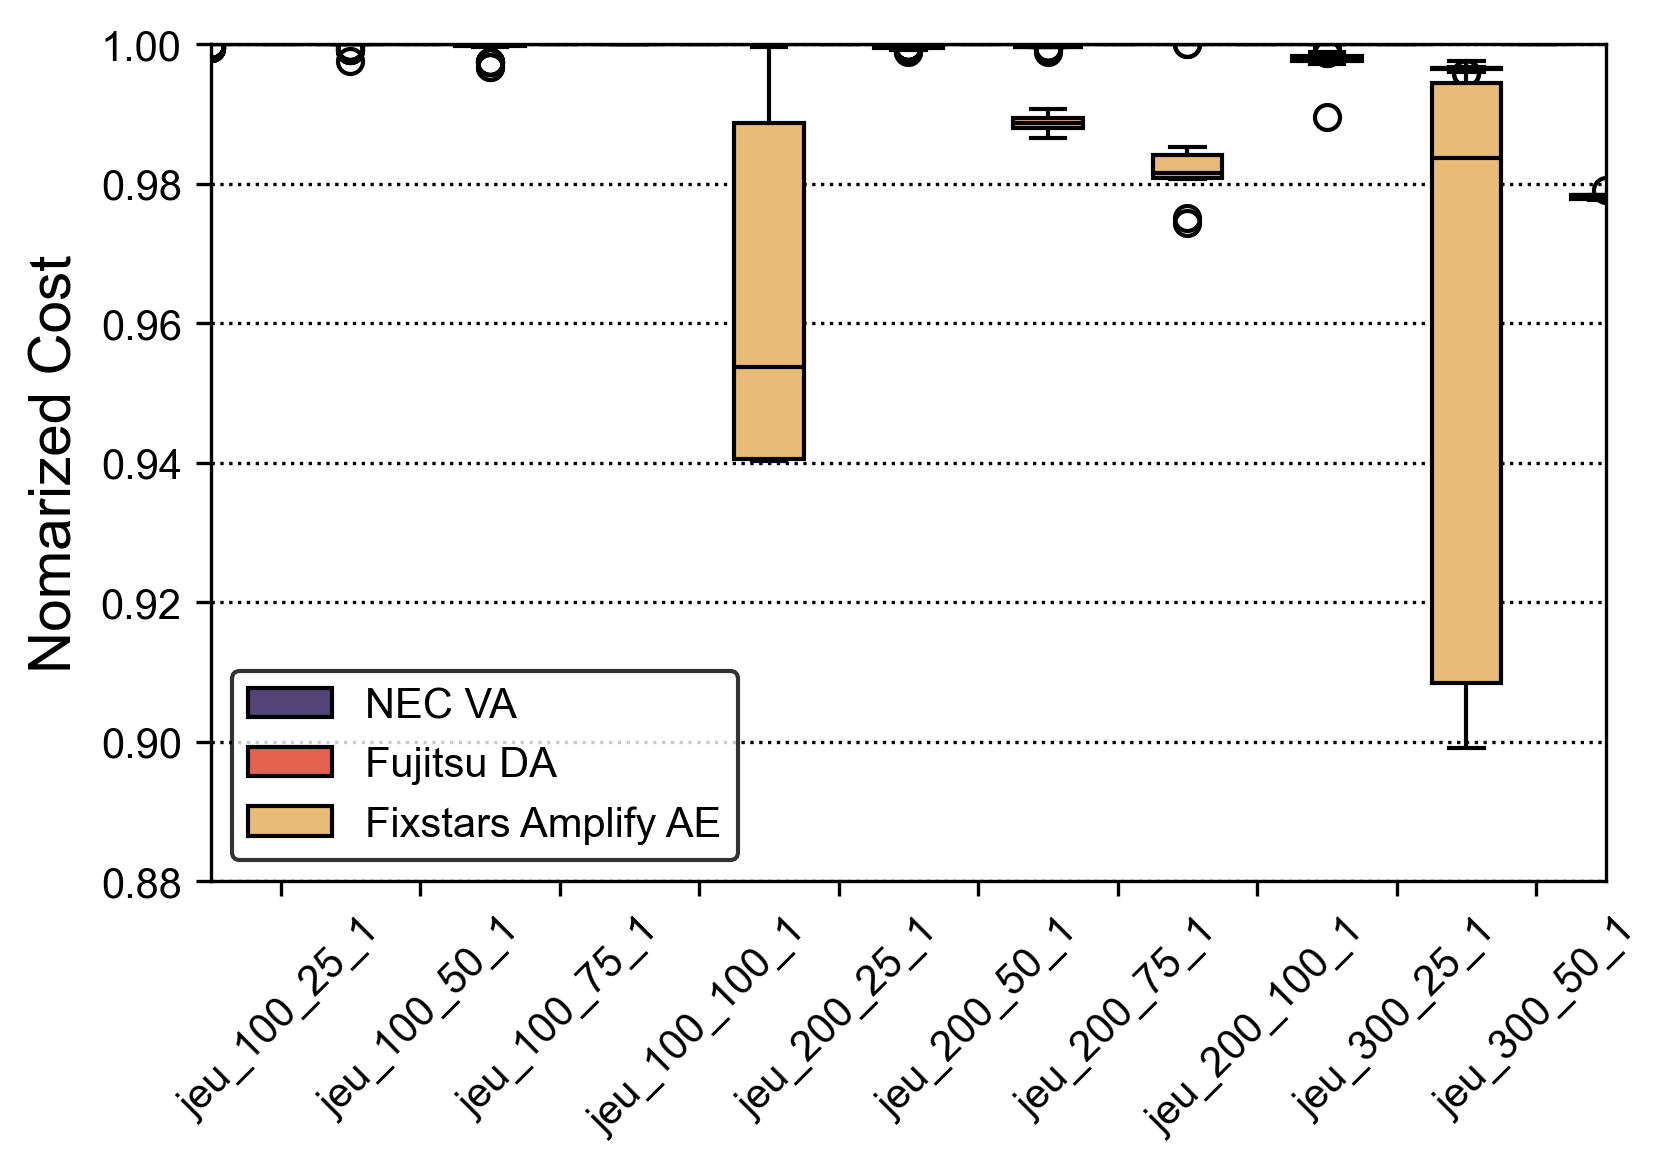
\includegraphics[bb=0 0 700 280, width=15cm]{speed_vs_constraint_QKP.png}
\caption{QKPにおけるNEC VAの2種類の制約機能の性能比較.}
\label{QKP_speed_vs_const}
\end{figure}
%4.2.4
\subsubsection{禁止ペア制約を持つMISによる評価}
% \textcolor{blue}{ベンチマークセットとして, BHOSLIB[YYY]のうち8つのインスタンスを用いた. 各インスタンス名のfrbに続く数値が大きくなるほど変数量が大きい. TTS計算の基準とする解精度は, 全てのインスタンスにおいて最適解とした. ソルバ毎の設定として, NEC VAではコア数を8, 始温度および終温度を10, num\_sweepsを1, andzeroフリップオプションを有効化, constraintモードによる実行とし, 富士通DAではtime\_limit\_secを5, target\_energyを最適解のエネルギー, 制約項をPenaltyBinaryPolynomialにより指定し, Fixstars Amplify AEではtimeoutを5000-600000(msec), 制約項の重みを1.0とした.}

図\ref{MIS_TTS}に, MISによるTTSの評価結果を示す. ベンチマークセットとして, BHOSLIB\cite{mislib}のうち8つのインスタンスを用いた. 各インスタンス名のfrbに続く数値が大きいほど変数量が大きい. 図\ref{MIS_TTS}より, frb40-19-1までの小中規模のインスタンスでは, NEC VA, Fixstars Amplify AE, Fujitsu DAの順に小さいTTSが得られている. 一方, Fujitsu DAでは問題サイズの増加に伴うTTSの増加が小さく, 最大のfrb100-40ではFujitsu DAが最小のTTSを達成している. また同図より, MISでは評価に用いた全てのソルバにおいて全インスタンスで最適解が得られていることが分かる. これは, 前述のワンホット制約, 不等式制約における各ソルバの性能傾向と比較すると, 標準的なFixstars Amplify AEを含む全てのソルバが高い求解性能を示していることを表す. 式(\ref{ham_mis})で示した通り, MISに含まれる禁止ペア制約は二つのバイナリ変数の積で構成されることから, 二次式であるQUBO表現と親和性が高く, エネルギー関数に自然にマップされる. このため, 制約をペナルティ関数として含めるFixstars Amplify AEにおいても高い求解性能を発揮したと考えられる. この検証として, NEC VAを用いて, フリップオプションを指定する場合と, フリップオプションを指定せず, 禁止ペア制約をペナルティ関数として導入した場合の性能差を確認する. 図\ref{MIS_speed_vs_const}に, MISの各インスタンスにおける, NEC VAのconstraintモードを指定する場合の実行時間と, フリップオプションを指定せず, 制約によるペナルティ関数をQUBOに含める場合の実行時間の比較を示す. ここで, 実行時間は, constraintモードを指定する場合の実行時間を1として全体の結果を正規化している. 図\ref{MIS_speed_vs_const}より, フリップオプションを指定しない場合, 全インスタンスにおいて, constraintモード実行による実行時間よりも短い実行時間を示していることが分かる. この要因として, 禁止ペア制約においては, 制約をQUBOに含めることによる実行時間や解精度への影響が比較的小さく, 一方フリップオプションを指定する場合においては, 外部入力された各制約を探索時に考慮する処理が加わる分, 一探索当たりの実行時間で遅延が発生することが影響していると考えられる.

\begin{figure}[hb]
\centering
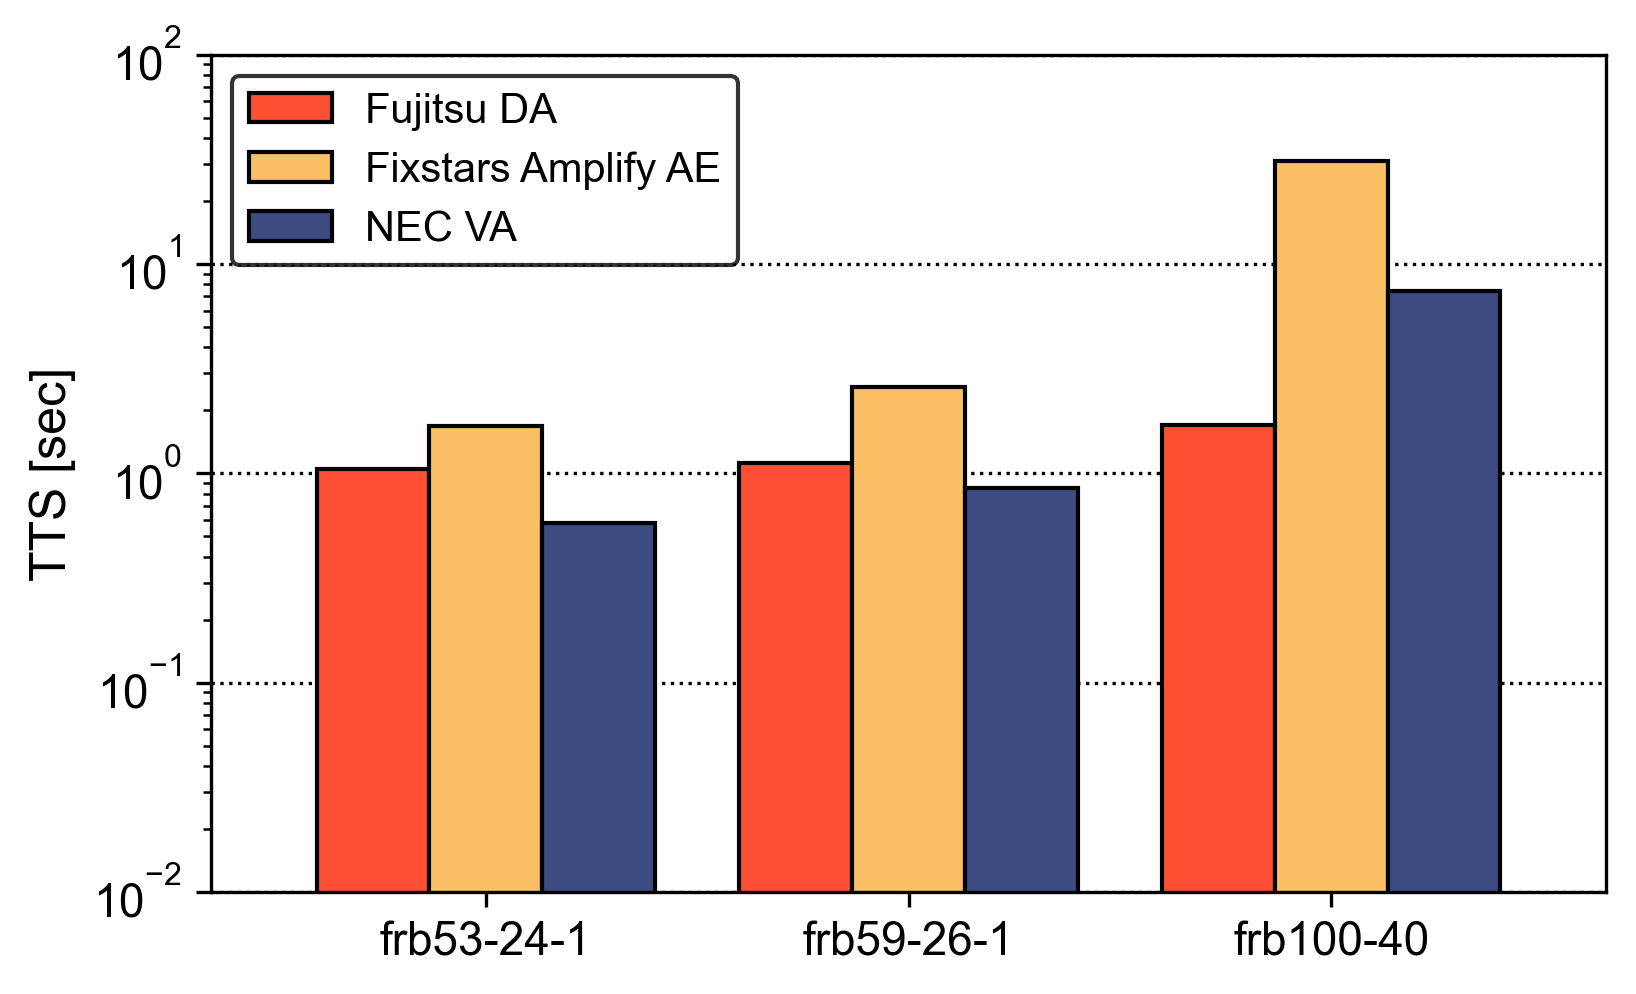
\includegraphics[bb=0 0 700 280, width=15cm]{TTS_MIS.png}
\caption{MISにおけるTTSの比較.}
\label{MIS_TTS}
\end{figure}

\begin{figure}[hb]
\centering
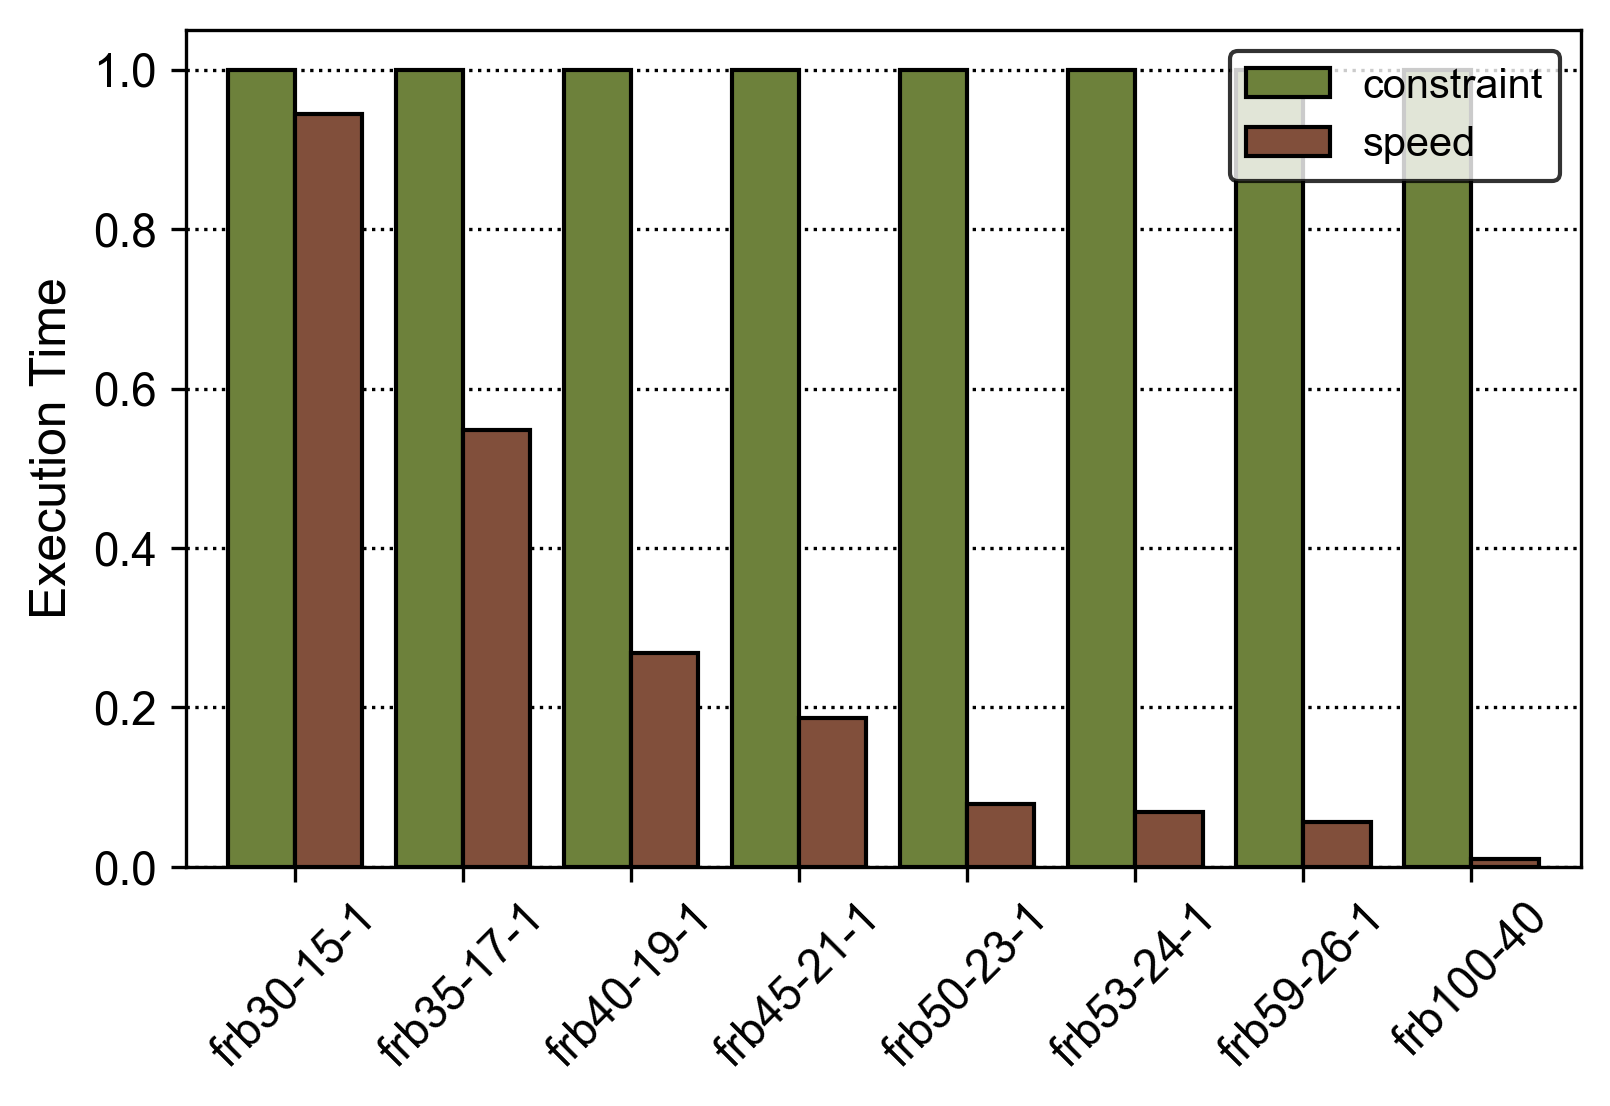
\includegraphics[bb=0 0 700 250, width=15cm]{speed_vs_constraint_MIS.png}
\caption{MISにおけるNEC VAの2種類の制約機能の性能比較.}
\label{MIS_speed_vs_const}
\end{figure}

%6
\section{おわりに}

本稿では,制約を含まないMaxcut, 及び異なる制約を含むTSP, QAP, QKP, MISを用いて, 擬似量子アニーリングマシンの制約機能の評価を行った. 結果として, 制約を含む最適化問題において, Fujitsu DA, NEC VAで制約機能を指定した場合, 標準的な疑似量子アニーリングマシンであるFixstars Amplify AEに対して高い性能を示すことが分かった. これは, 擬似量子アニーリングマシンにおいて, プラットフォームであるハードウェアの性能差以上に制約機能が全体の性能に大きく寄与していることを示唆している. さらに, 同じ制約を持つTSP, QAPにおいて, 類似の制約機能を持つFujitsu DA, NEC VAが異なる性能傾向を示す結果が確認された. このことから, 問題毎のQUBOによるエネルギー地形上の特性や各ソルバにおける制約機能の実装が結果に影響していることが明らかになった. 

\begin{acknowledgment}
本研究の一部は,文部科学省「次世代領域研究開発」(高性能汎用計算機高度利用事業費補助金)「量子アニーリングアシスト型次世代スーパーコンピューティング基盤の開発」,文部科学省「次世代計算基盤に係る調査研究」新計算原理調査研究,科研費基盤A\#19H01095,科研費基C\#20K11838,科研費特別研究員奨励費\#22J22908を受けて実施している.
\end{acknowledgment}

\begin{thebibliography}{10}

\bibitem{nishimori}
T. Kadowaki and H. Nishimori, “Quantum annealing in the transverse Ising model,” {\it Physical Review E}, 58, article number: 5355, 1998.

\bibitem{d-wave}
M. W. Johnson, {\it et al}. (2011). “Quantum annealing with manufactured spins”. {\it Nature} 473: 194–198.

\bibitem{takano}
鷹野芙美代, 鈴木基己, 小林悠記, 荒木拓也. 組合せ最適化問題における制約条件を考慮したQUBOソルバ, Vol. 119, No. 314(MSS2019 23-40), pp. 15-20, 2019.

\bibitem{Lucas} 
Andrew Lucas. Ising formulations of many np problems. {\it Frontiers in physics}, p. 5, 2014.

\bibitem{yatabe}
A. Yatabe, “Partitioning QUBO with two-way one-hot conditions on traveling salesman problems for city distributions with multiple clusters,” {\it Frontiers}, Vol. 6, 2024.

\bibitem{gset}
Gset. \urlj{https://web.stanford.edu/~yyye/yyye/Gset/.}

\bibitem{tsplib}
TSPLIB, \urlj{http://comopt.ifi.uni-heidelberg.de/software/TSPLIB95/.}

\bibitem{qaplib}
QAPLIB-Problem Instances and Solutions, \urlj{https://coral.ise.lehigh.edu/data-sets/qaplib/qaplib-
problem-instances-and-solutions/}

\bibitem{qkplib}
É. Soutif A. Billionnet. “An exact method based on Lagrangian decomposition for the 0–1 quadratic knapsack problems”. In: {\it Eur.J.Oper.Res.} Vol. 157. 3. 2024, pp. 565–575.

\bibitem{mislib}
BHOSLIB. \urlj{https://networkrepository.com/bhoslib.php}

\bibitem{va} 
NEC Corporation, "今ある最適化問題解決に - NEC Vector Annealing" \urlj{https://jpn.nec.com/nec-vector-annealing-service/index.html.}

\bibitem{da}
Tamura, H. and Katzgraber, H. G.: Physics-Inspired Optimization for Quadratic Unconstrained Problems Using a Digital Annealer, {\it Frontiers in Physics}, Vol. 7, No. 48, pp. 1–14 (2019).

\bibitem{amplify}
Fixstars Corporation, "Annealing Machines - The Quantum Computing Cloud - Fixstars Amplify." 
\urlj{https://amplify.fixstars.com/en/engine.}

\end{thebibliography}

\end{document}
